\setcounter{chapter}{3}
% \chapter{Quan hệ song song trong không gian}
\setcounter{section}{9}
\section{Đường thẳng và mặt phẳng trong không gian}
\subsection{Tóm tắt lý thuyết}
\subsubsection{Khái niệm mở đầu}
\begin{tcolorbox}[colback=orange!10!white]
\begin{itemize}
	\item Điểm $A$ thuộc mặt phẳng $(P)$, kí hiệu $A\in(P)$.
	\item Điểm $B$ không thuộc mặt phẳng $(P)$, kí hiệu $B\notin(P)$.\\
	Nếu $A\in(P)$ ta còn nói $A$ nằm trên $(P)$, hoặc $(P)$ chứa $A$, hoặc $(P)$ đi qua $A$.
\end{itemize}
\end{tcolorbox}
\begin{note}
	Để nghiên cứu hình học không gian, ta thường vẽ các hình đó lên bảng hoặc lên giấy. Hình vẽ đó được gọi là hình biểu diễn của một hình không gian. Hình biểu diễn của một hình không gian cần tuân thủ những quy tắc sau:\\
	\begin{minipage}{0.6\textwidth}
		\begin{itemize}
			\item Hình biểu diễn của đường thẳng là đường thẳng, của đoạn thẳng là đoạn thẳng.
			\item Hình biểu diễn của hai đường thẳng song song là hai đường thẳng cắt nhau là hai đường thẳng cắt nhau.
			\item Hình biểu diễn giữ nguyên quan hệ thuộc giữa điểm và đường thẳng.
			\item Dùng nét liền để biểu diễn cho đường nhìn thấy và nét đứt đoạn để biểu diễn cho đường bị che khuất.
		\end{itemize}
	\end{minipage}
\hspace{1cm}
\begin{minipage}{0.3\textwidth}
\begin{tikzpicture}[scale=1, line join=round, line cap=round]
	\coordinate (A) at (0,0);
	\coordinate (B) at (1,-0.5);
	\coordinate (C) at (2,0.5);
	\coordinate (D) at (0.8,2.5);
	\draw (A)--(B)--(C)--(D)--cycle;
	\draw (D)--(B);
	\draw[dashed] (A)--(C);
	\coordinate (A1) at (3,0);
	\coordinate (A2) at (5.0,0);
	\coordinate (A4) at (3.5,1.0);
	\coordinate (A3) at ($(A4)+(A2)-(A1)$);
	\foreach \x in {1,2,3,4} \coordinate (B\x) at ($(A\x)+(0,2)$);
	\draw (A1)--(A2)--(A3)--(B3)--(B4)--(B1)--cycle;
	\draw (B2)--(B3) (B2)--(B1) (B2)--(A2);
	\draw[dashed] (A4)--(A1) (A4)--(A3) (A4)--(B4);
\end{tikzpicture}
\textbf{Hình 4.3.} Hình biểu diễn của hình chóp tam giác đều và hình lập phương.
		
%		\caption{Hình biểu diễn của hình chóp tam giác đều và hình lập phương.}

\end{minipage}\\
	Các quy tắc khác sẽ được học ở phần sau.
\end{note}
\subsubsection{Các tính chất thừa nhận}
\begin{tcolorbox}[colback=orange!10!white,breakable]
	\begin{tc}
		Có một và chỉ một đường thẳng đi qua hai điểm phân biệt.
	\end{tc}
	\begin{tc}
		Có một và chỉ một mặt phẳng đi qua ba điểm không thẳng hàng.
	\end{tc}
	\begin{tc}
		Tồn tại bốn điểm không cùng thuộc một mặt phẳng.
	\end{tc}
	\begin{tc}
		Nếu một đường thẳng có hai điểm phân biệt cùng thuộc một mặt phẳng thì mọi điểm của đường thẳng đều thuộc mặt phẳng đó.
	\end{tc}
	\begin{tc}
		Nếu hai mặt phẳng phân biệt có một điểm chung thì chúng còn có một điểm chung khác nữa.\\
		Vậy thì: Nếu hai mặt phẳng phân biệt có một điểm chung thì chúng có một đường thẳng chung đi qua điểm chung ấy. Đường thẳng đó được gọi là giao tuyến của hai mặt phẳng.
	\end{tc}
	\begin{tc}
		Trên mỗi mặt phẳng, các kết quả đã biết trong hình học phẳng đều đúng.
	\end{tc}
\end{tcolorbox}
\subsubsection{Cách xác định mặt phẳng}
\begin{tcolorbox}[colback=orange!10!white,breakable]
Một mặt phẳng hoàn toàn xác định khi biết:
\begin{itemize}
	\item Nó đi qua ba điểm không thẳng hàng.
	\item Nó đi qua một điểm và một đường thẳng không đi qua điểm đó.
	\item Nó chứa hai đường thẳng cắt nhau.
\end{itemize}	
\end{tcolorbox}
Các kí hiệu:
\begin{itemize}
	\item $(ABC)$ là kí hiệu mặt phẳng đi qua ba điểm không thẳng hàng $A$, $B$, $C$.
	\item $(M,d)$ là kí hiệu mặt phẳng đi qua $d$ và điểm $M\notin d$.
	\item $(d_1,d_2)$ là kí hiệu mặt phẳng xác định bởi hai đường thẳng cắt nhau $d_1$, $d_2$.
\end{itemize}
\subsubsection{Hình chóp và hình tứ diện}
\begin{tcolorbox}[colback=orange!10!white,breakable]
\immini{Trong mặt phẳng $(\alpha)$ cho đa giác lồi $A_1A_2\ldots A_n$. Lấy điểm $S$ nằm ngoài $(\alpha)$. Lần lượt nối $S$ với các đỉnh $A_1$, $A_2$,$\ldots$, $A_n$ và $n$ tam giác $SA_1A_2$, $SA_2A_3$,$\ldots$,$SA_nA_1$ được gọi là hình chóp, kí hiệu là $S.A_1A_2\ldots A_n$.\\
Ta gọi:
\begin{itemize}
	\item $S$ là đỉnh;
	\item Đa giác $A_1A_2\ldots A_n$ là đáy;
	\item Các đoạn $SA_1$, $SA_2$,$\ldots$,$SA_n$ là các cạnh bên;
	\item Các đoạn $A_1A_2$, $A_2A_3$,$\ldots$,$A_nA_1$ là các cạnh đáy;
	\item Các tam giác $SA_1A_2$, $SA_2A_3$,$\ldots$,$SA_nA_1$ là các mặt bên.
\end{itemize}}{\begin{tikzpicture}[scale=0.8, line join=round, line cap=round]
	\coordinate (A) at (0,0);
	\coordinate (D) at (5.5,0);
	\coordinate (C) at (1,3);
	\coordinate (B) at ($(C)+(D)-(A)$);
	\coordinate (A1) at (1.5,2);
	\coordinate (A2) at (1.8,0.7);
	\coordinate (A3) at (2.5,0.5);
	\coordinate (A4) at (3.8,0.6);
	\coordinate (A5) at (4.6,1.1);
	\coordinate (A6) at (5.0,2.1);
	\coordinate (S) at (3,5);
	\coordinate (J) at (intersection of S--A6 and B--C);
	\coordinate (I) at (intersection of S--A1 and B--C);
	\draw (C)--(I) (J)--(B)--(D);
	\draw[dashed] (I)--(J);
	\draw pic["$P$", draw=black, angle eccentricity=.5, angle radius=0.6cm]
	{angle=D--A--C}; %góc
	\draw (A1)--(A2)--(A3)--(A4)--(A5)--(A6);
	\draw[dashed] (A1)--(A6);
	\draw (C)--(A)--(D);
	\foreach \x in {2,3,4,5} \draw (A\x) node[below]{$A\x$};
	\draw (A1) node[left]{$A_1$};
	\draw (A6) node[right]{$A_6$};
	\foreach \x in{1,2,3,4,5,6} \draw (S)--(A\x);
	\foreach \x in{1,2,3,4,5,6} \draw[fill=red] (A\x) circle (1pt);
	\draw[fill=red] (S) circle (1pt) node[above]{$S$};
\end{tikzpicture}}	
\end{tcolorbox}
\begin{tcolorbox}[colback=orange!10!white,breakable]
	\immini{Cho bốn điểm $A$, $B$, $C$, $D$ không đồng phẳng. Hình gồm bốn tam giác $ABC$, $ABD$, $ACD$ và $BCD$ được gọi là tứ diện $ABCD$.}{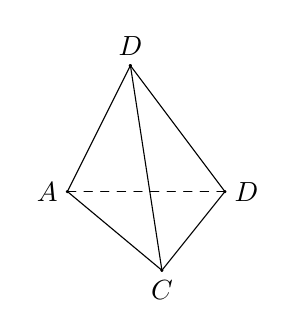
\begin{tikzpicture}[scale=0.4, line join=round, line cap=round]
			\coordinate (B) at (0,0);
			\coordinate (C) at (3,-2.5);
			\coordinate (D) at (5,0);
			\coordinate (A) at (2,4);
			\draw (A)--(B)--(C)--(D)--cycle;
			\draw (A)--(C);
			\draw[dashed] (B)--(D);
			\foreach \x in{A,B,C,D} \draw[fill=red] (\x) circle (1pt);
			\draw[fill=red] (A) circle (1pt) node[above]{$D$};
			\draw (B) node[left]{$A$};
			\draw (D) node[right]{$D$};
			\draw (C) node[below]{$C$};
	\end{tikzpicture}}
\end{tcolorbox}
\subsection{Hệ thống bài tập}
\begin{dang}{Tìm giao tuyến của hai mặt phẳng}
	Để xác định giao tuyến của hai mặt phẳng, ta tìm hai điểm chung của chúng. Đường thẳng đi qua hai điểm chung đó là giao tuyến.
	\begin{note}
		Lưu ý: Điểm chung của hai mặt phẳng $(\alpha)$ và $(\beta)$ thường được tìm như sau: Tìm hai đường thẳng $a$, $b$ lần lượt thuộc $(\alpha)$ và $(\beta)$, đồng thời chúng cùng nằm trong mặt phẳng $(\gamma)$ nào đó; giao điểm $M=a\cap b$ là điểm chung của $(\alpha)$ và $(\beta)$.
	\end{note}
\end{dang}
\subsubsection{Bài tập tự luận}
\begin{bt}%[1K4B0-3]
	Cho hình chóp $S.ABCD$, đáy $ABCD$ là tứ giác có các cặp cạnh đối không song song, điểm $M$ thuộc cạnh $SA$. Tìm giao tuyến của các cặp mặt phẳng:
	\begin{listEX}[2]
		\item $(SAC)$ và $(SBD)$.
		\item $(SAC)$ và $(MBD)$.
		\item $(MBC)$ và $(SAD)$.
		\item $(SAB)$ và $(SCD)$.
	\end{listEX}
\loigiai{
	\begin{enumerate}
		\item Gọi $O=AC\cap BD\Rightarrow\heva{&O\in AC\subset (SAC)\\&O\in BD\subset(SBD)}\Rightarrow O\in(SAC)\cap(SBD)$.\\
		Lại có $S\in(SAC)\cap(SBD)$.\\
		$\Rightarrow SO=(SAC)\cap(SBD)$.
		\item $O=AC\cap BD$ $\Rightarrow\heva{&O\in AC\subset (SAC)\\&O\in BD\subset(MBD)}\Rightarrow O\in(SAC)\cap(MBD)$.\\
		Và $M\in(SAC)\cap(MBD)\Rightarrow OM=(SAC)\cap(MBD)$.
		\item Trong $(ABCD)$, gọi $F=BC\cap AD\Rightarrow\heva{&F\in BC\subset(MBC)\\&F\in AD\subset(SAD)}\Rightarrow F\in(MBC)\cap(SAD)$.\\
		Và $M\in(MBC)\cap(SAD)\Rightarrow FM=(MBC)\cap(SAD)$.
		\item Trong $(ABCD)$, gọi $E=AB\cap CD$, ta có $SE=(SAB)\cap(SCD)$.
	\end{enumerate}
}
\end{bt}
\begin{bt}%[1K4B0-3]
	Cho hình chóp $S.ABCD$ có $AC\cap BD=M$ và $AB\cap CD=N$. Tìm giao tuyến của mặt phẳng $(SAC)$ và mặt phẳng $(SBD)$.
	\loigiai{
		\begin{center}
			\begin{tikzpicture}[scale=1, line join=round, line cap=round]
				\coordinate (A) at (0,0);
				\coordinate (D) at (5,0);
				\coordinate (N) at (2,-2);
				\coordinate (C) at ($(D)!0.6!(N)$);
				\coordinate (B) at ($(A)!0.7!(N)$);
				\coordinate (S) at (3,3);
				\draw (S)--(A)--(N)--(D)--cycle;
				\draw (S)--(B) (S)--(N) (S)--(C);
				\coordinate (M) at (intersection of A--C and B--D);
				\draw[dashed] (S)--(M) (A)--(C) (B)--(D) (A)--(D);
				\foreach \x in{A,B,C,D,N,S,M} \draw[fill=red] (\x) circle (1pt);
				\foreach \x in{A,B,B,N,D,C,M} \draw (\x) node[below]{$\x$};
				\draw (S) node[above]{$S$};
			\end{tikzpicture}
		\end{center}
		Ta có $(SAC)\cap(SBD)=SM$.
	}
\end{bt}
\begin{bt}%[1K4B0-3]
	Cho tứ diện $ABCD$. $G$ là trọng tâm tam giác $BCD$. Tìm giao tuyến của hai mặt phẳng $(ACD)$ và $(GAB)$.
	\loigiai{
		\immini{
		$A$ là điểm chung thứ nhất của $(ACD)$ và $(GAB)$.\\
		$G$ là trọng tâm tam giác $BCD$, $N$ là trung điểm $CD$ nên $N\in BG$ nên $N$ là điểm chung thứ hai của $(ACD)$ và $(GAB)$. Vậy giao tuyến của hai mặt phẳng $(ACD)$ và $(GAB)$ là $AN$.}{\begin{tikzpicture}[scale=1, line join=round, line cap=round]
			\coordinate (B) at (0,0);
			\coordinate (D) at (5,0);
			\coordinate (C) at (2,-2);
			\coordinate (A) at (1.5,3);
			\coordinate (N) at ($(C)!0.5!(D)$);
			\coordinate (G) at ($(B)!2/3!(N)$);
			\draw (A)--(B)--(C)--(D)--cycle;
			\draw (A)--(C) (A)--(N);
			\draw[dashed] (A)--(G) (B)--(N) (B)--(D);
			\foreach \x in{A,B,C,D,N,G} \draw[fill=red] (\x) circle (1pt);
			\foreach \x in{B,C,N,D,G} \draw (\x) node[below]{$\x$};
			\draw (A) node[above]{$A$};
	\end{tikzpicture}}
	}
\end{bt}
\begin{bt}%[1K4B0-3]
	Cho hình chóp $S.ABCD$. Gọi $I$ là trung điểm của $SD$, $J$ là điểm trên $SC$ và không trùng trung điểm $SC$. Tìm giao tuyến của hai mặt phẳng $(ABCD)$ và $(AIJ)$.
	\loigiai{
		\begin{center}
			\begin{tikzpicture}[scale=1, line join=round, line cap=round]
				\coordinate (A) at (0,0);
				\coordinate (D) at (6,0);
				\coordinate (B) at (0.6,-1);
				\coordinate (C) at (4,-2.0);
				\coordinate (S) at (2,4);
				\coordinate (I) at ($(S)!0.5!(D)$);
				\coordinate (J) at ($(S)!4/5!(C)$);
				\coordinate (F) at (intersection of D--C and I--J);
				\coordinate (M) at (intersection of B--C and A--F);
				\draw (S)--(A)--(B)--(S)--(J)--(F)--(D)--(S);
				\draw (S)--(B) (S)--(C) (F)--(I) (B)--(M)--(F);
				\draw[dashed] (A)--(M) (M)--(C) (A)--(J) (A)--(I) (A)--(D);
				\foreach \x in{A,B,C,D,S,I,J,F} \draw[fill=red] (\x) circle (1pt);
				\foreach \x in{B,F,C,D,A} \draw (\x) node[below]{$\x$};
				\draw (S) node[above]{$S$};
				\draw (I) node[above right]{$I$};
				\draw (J) node[right]{$J$};
			\end{tikzpicture}
		\end{center}
		$A$ là điểm chung thứ nhất của $(ABCD)$ và $(AIJ)$.\\
		$IJ$ và $CD$ cắt nhau tại $F$, còn $IJ$ không cắt $BC$, $AD$, $AB$ nên $F$ là điểm chung thứ hai của $(ABCD)$ và $(AIJ)$. Vậy giao tuyến của $(ABCD)$ và $(AIJ)$ là $AF$.
	}
\end{bt}
\begin{bt}%[1K4B0-3]
	Cho hình chóp $S.ABCD$ có đáy $ABCD$ là hình bình hành. Gọi $M$, $N$ lần lượt là trung điểm $AD$ và $BC$. Tìm giao tuyến của hai mặt phẳng $(SMN)$ và $(SAC)$.
	\loigiai{
		\begin{center}
			\begin{tikzpicture}[scale=1, line join=round, line cap=round]
				\coordinate (A) at (0,0);
				\coordinate (B) at (4,0);
				\coordinate (D) at (2,2);
				\coordinate (C) at ($(B)+(D)-(A)$);
				\coordinate (S) at (3,5);
				\coordinate (M) at ($(A)!0.5!(D)$);
				\coordinate (N) at ($(B)!0.5!(C)$);
				\coordinate (O) at (intersection of M--N and A--C);
				\draw (S)--(A)--(B)--(C)--cycle;
				\draw (S)--(B) (S)--(N);
				\draw[dashed] (A)--(D)--(C) (M)--(N) (S)--(M) (S)--(O) (S)--(D) (A)--(C);
				\foreach \x in{A,B,C,D,S,M,N,O} \draw[fill=red] (\x) circle (1pt);
				\foreach \x in{A,B,N,O,M,C,D} \draw (\x) node[below]{$\x$};
				\draw (S) node[above]{$S$};
			\end{tikzpicture}
		\end{center}
		$S$ là điểm chung thứ nhất của $(SMN)$ và $(SAC)$.\\
		$O$ là giao điểm của $AC$ và $MN$ nên $O\in AC$, $O\in MN$ do đó $O$ là điểm chung thứ hai của $(SMN)$ và $(SAC)$. Vậy giao tuyến của hai mặt phẳng $(SMN)$ và $(SAC)$ là $SO$.
	}
\end{bt}
\subsubsection{Bài tập trắc nghiệm}
\Opensolutionfile{ans}[ans/ans1C4B10-dang1]
\begin{ex}%[1K4B0-3]
	Cho hình chóp $S.ABCD$ có $AC\cap BD=M$ và $AB\cap CD=I$.\\
	Giao tuyến của hai mặt phẳng $(SAB)$ và mặt phẳng $(SCD)$ là đường thẳng:
	\choice
	{\True $SI$}
	{$SA$}
	{$MN$}
	{$SM$}
	\loigiai{
		\begin{center}
			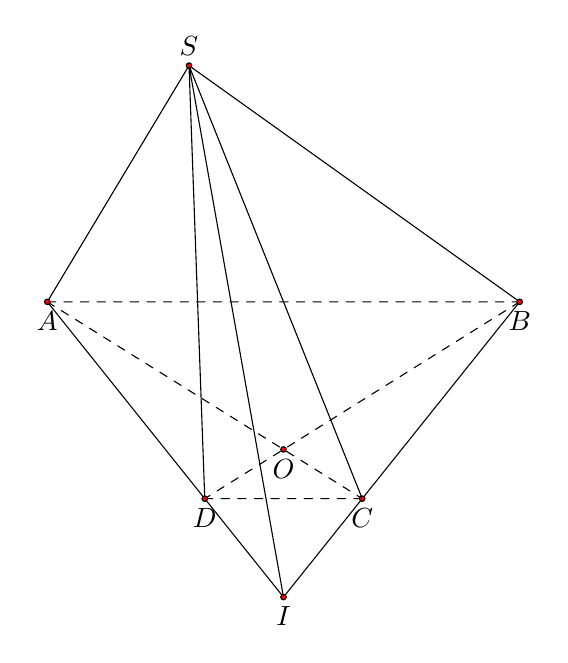
\begin{tikzpicture}[scale=1, line join=round, line cap=round]
				\coordinate (A) at (0,0);
				\coordinate (B) at (6,0);
				\coordinate (D) at (2,-2.5);
				\coordinate (C) at (4.0,-2.5);
				\coordinate (S) at (1.8,3);
				\coordinate (O) at (intersection of B--D and A--C);
				\coordinate (I) at (intersection of A--D and B--C);
				\draw (S)--(A)--(D)--(I)--(C)--(B)--cycle;
				\draw (S)--(D) (S)--(C) (S)--(I);
				\draw[dashed] (A)--(C) (B)--(D) (A)--(B) (C)--(D);
				\foreach \x in{A,B,C,D,I,O,S} \draw[fill=red] (\x) circle (1pt);
				\foreach \x in{A,D,I,C,B,O} \draw (\x) node[below]{$\x$};
				\draw (S) node[above]{$S$};
			\end{tikzpicture}
		\end{center}
		Ta có $(SAB)\cap(SCD)=SI$.
	}
\end{ex}
\begin{ex}
	Cho hình chóp $S.ABCD$ có đáy là hình thang $ABCD$ ($AB\parallel CD$).\\
	Khẳng định nào sau đây \textbf{sai}?
	\choice
	{Hình chóp $S.ABCD$ có $4$ mặt bên}
	{Giao tuyến của hai mặt phẳng $(SAC)$ và $(SBD)$ là $SO$ ($O$ là giao điểm của $AC$ và $BD$)}
	{Giao tuyến của hai mặt phẳng $(SAD)$ và $(SBC)$ là $SI$ ($I$ là giao điểm của $AD$ và $BC$)}
	{\True Giao tuyến của hai mặt phẳng $(SAB)$ và $(SAD)$ là đường trung bình của $ABCD$}
	\loigiai{
	\immini{\begin{itemize}
		\item Hình chóp $S.ABCD$ có $4$ mặt bên: $(SAB)$, $(SBC)$, $(SCD)$, $(SAD)$. Do đó $A$ đúng.
		\item $S$ là điểm chung thứ nhất của hai mặt phẳng $(SAC)$ và $(SBD)$.\\
		$\heva{&O\in AC\subset(SAC)\Rightarrow O\in(SAC)\\&O\in BD\subset(SBD)\Rightarrow O\in(SBD)}$ $\Rightarrow O$ là điểm chung thứ hai của hai mặt phẳng $(SAC)$ và $(SBD)$.\\
		$\Rightarrow (SAC)\cap (SBD)=SO$. Do đó B đúng.
		\item Tương tự, ta có $(SAD)\cap(SBC)=SI$. Do đó C đúng.
		\item $(SAB)\cap(SAD)=SA$ mà $SA$ không phải là đường trung bình của hình thang $ABCD$. Do đó $D$ sai.
	\end{itemize}}{\begin{tikzpicture}[scale=0.7, line join=round, line cap=round]
	\coordinate (A) at (0,0);
	\coordinate (B) at (7,0);
	\coordinate (D) at (1,-2.5);
	\coordinate (M) at ($(B)+(D)-(A)$);
	\coordinate (C) at ($(D)!0.5!(M)$);
	\coordinate (S) at (1.8,4);
	\coordinate (O) at (intersection of B--D and A--C);
	\coordinate (I) at (intersection of A--D and B--C);
	\draw (S)--(A)--(D)--(I)--(C)--(B)--cycle;
	\draw (S)--(D) (S)--(C) (S)--(I);
	\draw[dashed] (A)--(C) (B)--(D) (A)--(B) (C)--(D) (S)--(O);
	\foreach \x in{A,B,C,D,I,O,S} \draw[fill=red] (\x) circle (1pt);
	\foreach \x in{A,D,I,C,B,O} \draw (\x) node[below]{$\x$};
	\draw (S) node[above]{$S$};
\end{tikzpicture}}	
	}
\end{ex}
\begin{ex}%[1K4B0-3]
	Cho tứ diện $ABCD$. Gọi $G$ là trọng tâm của tam giác $BCD$. Giao tuyến của mặt phẳng $(ACD)$ và $(GAB)$ là
	\choice
	{$AM$ ($M$ là trung điểm của $AB$)}
	{\True $AN$ ($N$ là trung điểm của $CD$)}
	{$AH$ ($H$ là hình chiếu của $B$ trên $CD$)}
	{$AK$ ($K$ là hình chiếu của $C$ trên $BD$)}
	\loigiai{
		\immini{\begin{itemize}
			\item $A$ là điểm chung thứ nhất giữa hai mặt phẳng $(ACD)$ và $(GAB)$.
			\item Ta có $BG\cap CD=N\Rightarrow \heva{&N\in BG\subset (ABG)\Rightarrow N\in(ABG)\\&N\in CD\subset(ACD)\Rightarrow N\in (ACD)}$ $\Rightarrow N$ là điểm chung thứ hai giữa hai mặt phẳng $(ACD)$ và $(GAB)$.
		\end{itemize}
	Vậy $(ABG)\cap(ACD)=AN$.}{\begin{tikzpicture}[scale=0.6, line join=round, line cap=round]
		\coordinate (B) at (0,0);
		\coordinate (D) at (6,0);
		\coordinate (C) at (2,-2.5);
		\coordinate (N) at ($(C)!0.5!(D)$);
		\coordinate (G) at ($(B)!2/3!(N)$);
		\coordinate (A) at (2.5,4);
		\draw (A)--(B)--(C)--(D)--cycle;
		\draw (A)--(C) (A)--(N);
		\draw[dashed] (B)--(N) (A)--(G) (B)--(D);
		\foreach \x in{A,B,C,D,N,G} \draw[fill=red] (\x) circle (1pt);
		\foreach \x in{B,C,N,G,D} \draw (\x) node[below]{$\x$};
		\draw (A) node[above]{$A$};
\end{tikzpicture}}
	}
\end{ex}

\begin{ex}
	Cho hình chóp $S.ABCD$ có đáy $ABCD$ là hình bình hành. Gọi $I$, $J$ lần lượt là trung điểm của $SA$ và $SB$. Khẳng định nào sau đây \textbf{sai}?
	\choice
	{$IJCD$ là hình thang}
	{$(SAB)\cap(IBC)=IB$}
	{$(SBD)\cap(JCD)=JD$}
	{\True $(IAC)\cap(JBD)=AO$, $O$ là tâm hình bình hành $ABCD$}
	\loigiai{
	\immini{Ta có $(IAC)\equiv(SAC)$ và $(JBD)\equiv(SBD)$. Mà $(SAC)\cap(SBD)=SO$, trong đó $O$ là tâm hình bình hành $ABCD$.}{\begin{tikzpicture}[scale=0.6, line join=round, line cap=round]
			\coordinate (A) at (0,0);
			\coordinate (B) at (5,0);
			\coordinate (D) at (2,2.0);
			\coordinate (C) at ($(B)+(D)-(A)$);
			\coordinate (S) at (3,5);
			\coordinate (I) at ($(S)!0.5!(A)$);
			\coordinate (J) at ($(S)!0.5!(B)$);
			\coordinate (O) at (intersection of A--C and B--D);
			\draw (S)--(A)--(B)--(C)--cycle;
			\draw (S)--(B) (I)--(J)--(C);
			\draw[dashed] (S)--(D)--(A)--(C) (B)--(D) (I)--(D)--(C);
			\foreach \x in{A,B,C,D,O,I,J,S} \draw[fill=red] (\x) circle (1pt);
			\foreach \x in{A,B,C,D,O} \draw (\x) node[below]{$\x$};
			\draw (S) node[above]{$S$};
			\draw (I) node[above left]{$I$};
			\draw (J) node[above right]{$J$};
	\end{tikzpicture}}	
	}
\end{ex}

\begin{ex}%[1K4B0-3]
	Cho điểm $A$ không nằm trên mặt phẳng $(\alpha)$ chứa tam giác $BCD$. Lấy $E$, $F$ là các điểm lần lượt nằm trên các cạnh $AB$, $AC$. Khi $EF$ và $BC$ cắt nhau tại $I$ thì $I$ không phải là điểm chung của hai mặt phẳng nào sau đây?
	\choice
	{$(BCD)$ và $(DEF)$}
	{$(BCD)$ và $(ABC)$}
	{$(BCD)$ và $(AEF)$}
	{\True $(BCD)$ và $(ABD)$}
	\loigiai{
		\immini{Điểm $I$ là giao điểm của $EF$ và $BC$. \\
		Ta có $\heva{&EF\subset(DEF)\\&EF\subset(ABC)\\&EF\subset(AEF)}\Rightarrow \heva{&I=(BCD)\cap(DEF)\\&I=(BCD)\cap(ABC)\\&I=(BCD)\cap(AEF).}$}{
			\begin{tikzpicture}[scale=0.6, line join=round, line cap=round]
				\coordinate (B) at (0,0);
				\coordinate (D) at (5,0);
				\coordinate (A) at (2.5,4);
				\coordinate (C) at (2,-2.0);
				\coordinate (E) at ($(A)!0.6!(B)$);
				\coordinate (F) at ($(A)!4/5!(C)$);
				\coordinate (I) at (intersection of B--C and E--F);	
				\coordinate (M) at (intersection of D--C and I--F);	
				\draw (A)--(B)--(C)--(I)--(F)--(D)--(A)--(C);
				\draw (E)--(F) (M)--(D);
				\draw[dashed] (E)--(D) (C)--(M) (B)--(D);
				\foreach \x in{A,B,C,D,E,F,I} \draw[fill=red] (\x) circle (1pt);
				\foreach \x in{B,C,I,D} \draw (\x) node[below]{$\x$};
				\draw (A) node[above]{$A$};
				\draw (E) node[above left]{$E$};
				\draw (F) node[left]{$F$};
		\end{tikzpicture}}
	}
\end{ex}

\begin{ex}%[1K4B0-3]
Cho tứ diện $ABCD$. Gọi $M$, $N$ lần lượt là trung điểm của $AC$, $CD$. Giao tuyến của hai mặt phẳng $(MBD)$ và $(ABN)$ là
\choice
{Đường thẳng $MN$}
{Đường thẳng $AM$}
{Đường thẳng $BG$ ($G$ là trọng tâm tam giác $ACD$)}
{Đường thẳng $AH$ ($H$ là trực tâm tam giác $ACD$)}
\loigiai{
	\immini{\begin{itemize}
		\item $B$ là điểm chung thứ nhất giữa hai mặt phẳng $(MBD)$ và $(ABN)$.
		\item Vì $M$, $N$ lần lượt là trung điểm của $AC$, $CD$ nên suy ra $AN$, $DM$ là hai trung tuyến của tam giác $ACD$. Gọi $G=AN\cap DM$.\\
		$\Rightarrow\heva{&G\in AN\subset(ABN)\Rightarrow G\in(ABN)\\&G\in DM\subset (MBD)\Rightarrow G\in (MBD)}$ $\Rightarrow G$ là điểm chung thứ hai giữa hai mặt phẳng $(MBD)$ và $(ABN)$.\\
		Vậy $(ABN)\cap(MBD)=BG$.
	\end{itemize}}{\begin{tikzpicture}[scale=1, line join=round, line cap=round]
	\coordinate (B) at (0,0);
	\coordinate (D) at (5,0);
	\coordinate (C) at (3,-2.0);
	\coordinate (A) at (2,4);
	\coordinate (M) at ($(A)!0.5!(C)$);
	\coordinate (N) at ($(C)!0.5!(D)$);
	\coordinate (G) at (intersection of A--N and M--D);	
	\draw (A)--(B)--(C)--(D)--cycle;
	\draw (A)--(C) (A)--(N) (M)--(D) (B)--(M);
	\draw[dashed] (B)--(G) (B)--(N) (B)--(D);
	\foreach \x in{A,B,C,D,M,N,G} \draw[fill=red] (\x) circle (1pt);
	\foreach \x in{B,C,D,N} \draw (\x) node[below]{$\x$};
	\draw (A) node[above]{$A$};
	\draw (M) node[above right]{$M$};
	\draw (G) node[above right]{$G$};
\end{tikzpicture}}
}
\end{ex}
\Closesolutionfile{ans}
\begin{dang}{Tìm giao điểm của đường thẳng và mặt phẳng}
	Để tìm giao điểm của đường thẳng $d$ và mặt phẳng $(P)$ ta cần lưu ý một số trường hợp sau:\\
	\textbf{Trường hợp 1.} Nếu trong $(P)$ có sẵn một đường thẳng $d'$ cắt $d$ tại $M$, khi đó
	\[
	\heva{&M\in d\\&M\in d'\subset (P)}\Rightarrow \heva{&M\in d\\&M\in(P)}\Rightarrow M=d\cap (P).
	\]
	\immini{\textbf{Trường hợp 2.} Nếu trong $(P)$ chưa có sẵn $d'$ cắt $d$ thì ta thực hiện theo các bước sau:
	\begin{itemize}
		\item Bước 1: Chọn một mặt phẳng $(Q)$ chứa $d$.
		\item Bước 2: Tìm giao tuyến $\Delta=(P)\cap(Q)$.
		\item Bước 3: Trng $(Q)$ gọi $M=d\cap \Delta$ thì $M$ chính là giao điểm của $d\cap(P)$.
		
	\end{itemize}}{\begin{tikzpicture}[scale=1, line join=round, line cap=round]
	\coordinate (A) at (0,0);
	\coordinate (B) at (4,0);
	\coordinate (D) at (2,3);
	\coordinate (C) at ($(B)+(D)-(A)$);
	\coordinate (E) at ($(A)!0.6!(D)$);
	\coordinate (F) at ($(B)!0.4!(C)$);
	\coordinate (G) at (3.5,4);
	\coordinate (H) at ($(E)+(G)-(F)$);
	\draw (E)--(A)--(B)--(F)--cycle;
	\draw (E)--(F)--(G)--(H)--cycle;
	\coordinate (I) at (intersection of F--G and C--D);`
	\draw (I)--(C)--(F);
	\draw[dashed] (E)--(D)--(I);
	\draw pic["$P$", draw=black, angle eccentricity=.7, angle radius=1cm]
	{angle=E--H--G}; %góc
	\draw pic["$Q$", draw=black, angle eccentricity=.7, angle radius=1cm]
	{angle=B--A--E}; %góc
	\coordinate (M) at ($(E)!0.6!(F)$);
	\coordinate (N) at ($(G)!0.4!(H)$);
	\coordinate (U) at ($(N)!0.2!(M)$);
	\coordinate (V) at ($(N)!1.3!(M)$);
	\coordinate (W) at ($(E)!0.5!(M)$);
	\draw (W) node[below]{$d'$};
	\draw (U)--(M);
	\draw[dashed] (M)--(V);
	\foreach \x in{M} \draw[fill=red] (\x) circle (1pt);
	\draw (U)--(M) node[midway]{$\quad d$};
	\draw (M) node[below left]{$M$};
\end{tikzpicture}}
\end{dang}
\subsubsection{Bài tập tự luận}
\begin{bt}%[1K4B0-4]
	Cho bốn điểm $A$, $B$, $C$, $D$ không đồng phẳng. Gọi $M$, $N$ lần lượt là trung điểm của $AC$ và $BC$. Trên đoạn $BD$ lấy điểm $P$ sao cho $BP=2PD$. Tìm giao điểm của đường thẳng $CD$ và mặt phẳng $(MNP)$.
	\loigiai{
		\immini{\textbf{Cách 1.} Xét mặt phẳng $(BCD)$ chứa $CD$.\\
		Do $NP$ không song song $CD$ nên $NP$ cắt $CD$ tại $E$.\\
		Điểm $E\in NP\Rightarrow (MNP)$. Vậy $CD\cap(MNP)$ tại $E$.\\
		\textbf{Cách 2.} Ta có $\heva{&N\in BC\\&P\in BD}\Rightarrow NP\subset (MNP)$, suy ra $NP$, $CD$ đồng phẳng.\\
		Gọi $E$ là giao điểm của $NP$ và $CD$ mà $NP\subset(MNP)$ suy ra $CD\cap(MNP)=E$.\\
		Vậy giao điểm của $CD$ và mp$(MNP)$ là giao điểm $E$ của $NP$ và $CD$.}{\begin{tikzpicture}[scale=0.8, line join=round, line cap=round]
			\coordinate (B) at (0,0);
			\coordinate (D) at (6,0);
			\coordinate (C) at (3,-2.5);
			\coordinate (A) at (2,4);
			\coordinate (M) at ($(A)!0.5!(C)$);
			\coordinate (N) at ($(B)!0.5!(C)$);
			\coordinate (P) at ($(B)!2/3!(D)$);
			\coordinate (E) at (intersection of N--P and C--D);`
			\coordinate (I) at (intersection of A--D and M--E);`
			\draw (A)--(B)--(C)--cycle (A)--(D) (M)--(E) (M)--(N) (C)--(D)--(E);
			\draw[dashed] (M)--(P) (P)--(E) (P)--(I) (P)--(N) (B)--(D);
			\foreach \x in{A,B,C,D,M,N,E,I} \draw[fill=red] (\x) circle (1pt);
			\foreach \x in{B,C,D,N} \draw (\x) node[below]{$\x$};
			\draw (A) node[above]{$A$};
			\draw (E) node[right]{$E$};
			\draw (M) node[left]{$M$};
			\draw (P) node[below]{$P$};
	\end{tikzpicture}}
	}
\end{bt}
%%==========Bài 1
\begin{bt}%[1K4B0-4]
	Cho tứ giác $A B C D$ có $A C$ và $B D$ giao nhau tại $O$ và một điểm $S$ không thuộc mặt phẳng $(A B C D)$. Trên đoạn $S C$ lấy một điểm $M$ không trùng với $S$ và $C$. Tìm giao điểm của đường thẳng $S D$ với mặt phẳng $(A B M)$.
	\loigiai
	{
		\begin{center}
			\begin{tikzpicture}[line join = round, line cap = round,>=stealth,font=\footnotesize,scale=1]
				\def\ab{2} \def\ad{5} \def\bc{2.5}
				\def\goca{-60} \def\so{5}
				\path (0,0) coordinate (A)
				(\goca:\ab) coordinate (B)
				($(B)+(-15:\bc)$) coordinate (C)
				(\ad,0) coordinate (D)
				(intersection of A--C and B--D) coordinate (O)
				($(O)+(0,\so)$) coordinate (S)
				($(S)!.4!(C)$) coordinate (M)
				($(S)!.2!(D)$) coordinate (N)
				(intersection of A--M and B--N) coordinate (K)
				;
				\draw (A)--(B)--(C)--(D) (A)--(S)--(D) (B)--(S)--(C);
				\draw[dashed] (C)--(A)--(D)--(B) (S)--(O) (A)--(M) (B)--(N);	
				\foreach \x/\gm in {A/180,B/-120,C/-90,D/20,S/90,N/20,M/0,K/120,O/-90} \fill (\x) circle (1pt) ($(\x)+(\gm:3.5mm)$)node{$\x$};
			\end{tikzpicture}
		\end{center}
		\begin{itemize}
			\item [\color{teal}\faCheckCircleO] Chọn mặt phẳng phụ $(S B D)$ chứa $S D$.
			\item [\color{teal}\faCheckCircleO] Tìm giao tuyến của hai mặt phẳng $(S B D)$ và $(A B M)$.
		\end{itemize}
		Ta có $B$ là điểm chung thứ nhất của $(S B D)$ và $(A B M)$.\\
		Trong mặt phẳng $(A B C D)$, gọi $O=A C \cap B D$.\\
		Trong mặt phẳng $(S A C)$, gọi $K=A M \cap S O$.\\
		Khi đó $(S B D) \cap(A B M)=B K$.\\
		Trong $(S B D)$ lấy $N=B K \cap S D$ thì $N=S D \cap(A B M)$.	
	}
\end{bt}
%%==========Bài 2
\begin{bt}%[1K4B0-4]
	Cho hình chóp tứ giác $S . A B C D$ với đáy $A B C D$ có các cạnh đối diện không song song với nhau và $M$ là một điểm trên cạnh $S A$.
	\begin{enumerate}[a)]
		\item Tìm giao điểm của đường thẳng $S B$ với mặt phẳng $(M C D)$.
		\item Tìm giao điểm của đường thẳng $M C$ và mặt phẳng $(S B D)$.
	\end{enumerate}
	\loigiai
	{
		\immini
		{
			\begin{enumerate}[a)]
				\item Trong mặt phẳng $(ABCD)$, gọi $E=AB\cap CD$.\\
				Trong $(SAB)$ ta có $N\in EM\subset(MCD)\Rightarrow N\in(MCD)$ và $N\in SB$ nên $N=SB\cap(MCD)$.
				\item Trong $(ABCD)$ gọi $I=AC\cap BD$.\\
				Trong $(SAC)$ gọi $K=MC\cap SI$.\\
				Ta có $K\in SI\subset(SBD)$ và $K\in MC$ nên $K=MC\cap(SBD)$.
			\end{enumerate}
		}
		{
			\begin{tikzpicture}[line join = round, line cap = round,>=stealth,font=\footnotesize,scale=1]
				\def\ab{2} \def\ad{5} \def\bc{2.5}
				\def\goca{-60} \def\so{5}
				\path (0,0) coordinate (A)
				(\goca:\ab) coordinate (B)
				($(B)+(-15:\bc)$) coordinate (C)
				(\ad,0) coordinate (D)
				(intersection of A--C and B--D) coordinate (I)
				(intersection of A--B and D--C) coordinate (E)
				($(I)+(0,\so)$) coordinate (S)
				($(S)!.6!(A)$) coordinate (M)
				(intersection of E--M and S--B) coordinate (N)
				(intersection of S--I and C--M) coordinate (K)
				;
				\draw (S)--(A)--(E)--(D)--cycle
				(B)--(S)--(C) (M)--(E)
				;
				\draw[dashed] (M)--(D)--(A)--(C) (B)--(D) (S)--(I) (B)--(C)--(M);
				\foreach \x/\gm in {S/90,A/180,B/-150,E/-90,C/-50,D/0,K/0,M/180,N/180,I/-90} \fill (\x) circle (1pt) ($(\x)+(\gm:3.5mm)$)node{$\x$};	
			\end{tikzpicture}	
		}	
	}
\end{bt}
%%==========Bài 3
\begin{bt}%[1K4B0-4]
	Cho hình chóp tứ giác $S . A B C D, M$ là một điểm trên cạnh $S C, N$ là trên cạnh $B C$. Tìm giao điểm của đường thẳng $S D$ với mặt phẳng $(A M N)$.
	\loigiai
	{
		\immini
		{
			Trong mặt phẳng $(A B C D)$ gọi
			$O=A C \cap B D, J=A N \cap B D$.\\
			Trong $(S A C)$ gọi $I=S O \cap A M$ và $K=I J \cap S D$.\\
			Ta có $I \in A M \subset(A M N), J \in A N \subset(A M N)
			\Rightarrow I J \subset(A M N)$.\\
			Do đó $K \in I J \subset(A M N) \Rightarrow K \in(A M N)$.\\
			Vậy $K=S D \cap(A M N)$	
		}
		{
			\begin{tikzpicture}[line join = round, line cap = round,>=stealth,font=\footnotesize,scale=1]
				\def\ad{2} \def\ab{5} \def\cd{2.5}
				\def\goca{-60} \def\so{5}
				\path 
				(0,0) coordinate (A)
				(\goca:\ad) coordinate (D)
				($(D)+(-5:\cd)$) coordinate (C)
				(\ab,0) coordinate (B)
				(intersection of A--C and B--D) coordinate (O)
				($(S)!.6!(C)$) coordinate (M)
				($(C)!.7!(B)$) coordinate (N)
				(intersection of A--M and S--O) coordinate (I)
				(intersection of A--N and B--D) coordinate (J)
				(intersection of J--I and S--D) coordinate (K)
				;
				\draw (S)--(A)--(D)--(C)--(B)--cycle
				(D)--(S)--(C) (M)--(N)
				;
				\draw[dashed] (M)--(A)--(N) (S)--(O) (A)--(C) (B)--(D) (K)--(J) (A)--(B);
				\foreach \x/\gm in {A/180,B/0,C/-90,D/-90,J/-90,M/20,N/-10,K/180,I/50,S/90,O/-90} \fill (\x) circle (1pt) ($(\x)+(\gm:3.5mm)$)node{$\x$};	
			\end{tikzpicture}	
		}
	}
\end{bt}
%%==========Bài 4
\begin{bt}%[1K4B0-4]
	Cho hình chóp $S A B C D$ có đáy $A B C D$ là hình bình hành. Gọi $M, P$ lần lượt là trung điềm của các cạnh $S A$ và $S C$. Điểm $N$ thuộc cạnh $S B$ sao cho $\dfrac{S N}{S B}=\dfrac{2}{3}$. Gọi $Q$ là giao điểm của cạnh $S D$ và mặt phẳng $(M N P)$. Tính tỷ số $\dfrac{S Q}{S D}$.
	\loigiai
	{
		\immini
		{
			Gọi $O$ là giao điểm của $A C$ và $B D, I$ là giao điểm của $M P$ và $S O$ thì $Q$ là giao điểm của $N I$ với $S D . I$ là trung điểm của $S O$.\\
			Đặt $\dfrac{S D}{S Q}=x$.\\
			Do $2 \vv{S O}=\vv{S B}+\vv{S D}$ nên $4 \vv{S I}=\dfrac{3}{2} \vv{S N}+x \vv{S Q} \Rightarrow x=4-\dfrac{3}{2}=\dfrac{5}{2}$.\\
			Vậy $\dfrac{S Q}{S D}=\dfrac{2}{5}$.	
		}
		{
			\begin{tikzpicture}[scale=1, font=\footnotesize, line join=round, line cap=round, >=stealth]
				\def\bc{4} % cạnh BC
				\def\ba{2} % cạnh BA
				\def\h{4} % đường cao
				\def\gocB{30} % góc B của đáy
				\coordinate[label=below left:$B$] (B) at (0,0);
				\coordinate[label=above left:$A$] (A) at (\gocB:\ba);
				\coordinate[label=below:$C$] (C) at (\bc,0);
				\coordinate[label=right:$D$] (D) at ($(C)-(B)+(A)$);
				\coordinate[label=above:$S$] (S) at ($(A)+(80:\h)$);
				\path 
				($(S)!2/3!(B)$) coordinate (N)
				($(S)!0.5!(A)$) coordinate (M)
				($(S)!0.5!(C)$) coordinate (P)
				(intersection of A--C and B--D) coordinate (O)
				(intersection of M--P and S--O) coordinate (I)
				(intersection of S--D and N--I) coordinate (Q)
				;
				\draw (B)--(C)--(D)--(S)--cycle (S)--(C) (N)--(P)--(Q);
				\draw[dashed] (A)--(D) (S)--(A)--(B) (N)--(M)--(Q) (N)--(Q) (M)--(P) (A)--(C) (B)--(D) (S)--(O);
				\foreach \diem in {A,B,C,D,S}	\fill (\diem)circle(1.5pt);
				\foreach \x/\gm in {M/170,Q/20,N/180,P/0,I/190,O/-90} \fill (\x) circle (1pt) ($(\x)+(\gm:3.5mm)$)node{$\x$};
			\end{tikzpicture}	
		}
	}
\end{bt}
\subsubsection{Bài tập trắc nghiệm}
\Opensolutionfile{ans}[ans/ans1C4B10-dang2]
%%==========Câu 1
\begin{ex}%[1K4B0-4]
	Cho tứ diện $A B C D$. Gọi $E$ và $F$ lần lượt là trung điểm của $A B$ và $C D$; $G$ là trọng tâm tam giác $B C D$. Giao điểm của đường thẳng $E G$ và mặt phẳng $(A C D)$ là
	\choice
	{điểm $F$}
	{\True giao điểm của đường thẳng $E G$ và $A F$}
	{giao điểm của đường thẳng $E G$ và $A C$}
	{giao điểm của đường thẳng $E G$ và $C D$}
	\loigiai
	{
		\immini
		{
			Vì $G$ là trọng tâm tam giác $B C D$, $F$ là trung điểm của $C D \Rightarrow G \in(A B F)$.\\
			Ta có $E$ là trung điểm của $A B \Rightarrow E \in(A B F)$.\\
			Gọi $M$ là giao điểm của $E G$ và $A F$ mà $A F \subset(A C D)$ suy ra $M \in(A C D)$.\\
			Vậy giao điểm của $E G$ và $m p(A C D)$ là giao điểm $M=E G \cap A F$.	
		}
		{
			\begin{tikzpicture}[line join = round, line cap = round, thick, font = \small, scale = 1]
				\path 
				(0:0) coordinate (B)
				+(0:5) coordinate (D)
				+(-65:3) coordinate (C)
				(barycentric cs:B=1,C=1,D=1) coordinate (G)
				++(90:4) coordinate (A)
				($(A)!.5!(B)$) coordinate (E)
				($(C)!.5!(D)$) coordinate (F)
				(intersection of E--G and A--F) coordinate (M)
				(intersection of E--G and C--D) coordinate (em)
				;
				\draw[dashed] 
				(B)--(D) (E)--(em) (B)--(F)
				;
				\draw 
				(A)--(B)--(C)--(D)--cycle
				(A)--(C) (A)--(M)--(em) 
				;
				\foreach \x/\g in {B/180,C/-90,D/-90,A/90,E/160,F/-10,G/-110,M/0}
				\fill (\x) circle (1.5pt)
				+(\g:3.5mm) node {$\x$};
			\end{tikzpicture}	
		}	
	}
\end{ex}
%%==========Câu 2
\begin{ex}%[1K4B0-4]
	Cho hình chóp tứ giác $S A B C D$ với đáy $A B C D$ có các cạnh đối diện không song song với nhau và $M$ là một điểm trên cạnh $S A$. Tìm giao điểm của đường thẳng $S B$ với mặt phẳng $(M C D)$.
	\choice
	{Điểm $H$, trong đó $E=A B \cap C D, H=S A \cap E M$}
	{Điểm $N$, trong đó $E=A B \cap C D, N=S B \cap E M$}
	{Điểm $F$, trong đó $E=A B \cap C D, F=S C \cap E M$}
	{Điểm $T$, trong đó $E=A B \cap C D, T=S D \cap E M$}
	\loigiai
	{
		\immini
		{
			Trong mặt phẳng $(ABCD)$, gọi $E=AB\cap CD$.\\
			Trong $(SAB)$: ta có $N\in EM\subset(MCD)\Rightarrow N\in (MCD)$ và $N\in SB$ nên $N=SB\cap(MCD)$.	
		}
		{
			\begin{tikzpicture}[line join = round, line cap = round,>=stealth,font=\footnotesize,scale=1]
				\def\ab{2} \def\ad{5} \def\bc{2.5}
				\def\goca{-60} \def\so{5}
				\path (0,0) coordinate (A)
				(\goca:\ab) coordinate (B)
				($(B)+(-15:\bc)$) coordinate (C)
				(\ad,0) coordinate (D)
				(intersection of A--C and B--D) coordinate (I)
				(intersection of A--B and D--C) coordinate (E)
				($(I)+(0,\so)$) coordinate (S)
				($(S)!.6!(A)$) coordinate (M)
				(intersection of E--M and S--B) coordinate (N)
				(intersection of S--I and C--M) coordinate (K)
				;
				\draw (S)--(A)--(E)--(D)--cycle
				(B)--(S)--(C) (M)--(E)
				;
				\draw[dashed] (M)--(D)--(A)--(C) (B)--(D) (S)--(I) (B)--(C)--(M);
				\foreach \x/\gm in {S/90,A/180,B/-150,E/-90,C/-50,D/0,K/0,M/180,N/180,I/-90} \fill (\x) circle (1pt) ($(\x)+(\gm:3.5mm)$)node{$\x$};	
			\end{tikzpicture}	
		}	
	}
\end{ex}
%%==========Câu 3
\begin{ex}%[1K4B0-4]
	Cho hình chóp tứ giác $S A B C D$ với đáy $A B C D$ có các cạnh đối diện không song song với nhau và $M$ là một điểm trên cạnh $S A$. Tìm giao điểm của đường thẳng $M C$ và mặt phẳng $(S B D)$.
	\choice
	{Điểm $H$, trong đó $I=A C \cap B D$, $H=M A \cap S I$}
	{Điểm $F$, trong đó $I=A C \cap B D$, $F=M D \cap S I$}
	{Điểm $K$, trong đó $I=A C \cap B D$, $K=M C \cap S I$}
	{Điểm $V$, trong đó $I=A C \cap B D$, $V=M B \cap S I$}
	\loigiai
	{
		\immini
		{
			Trong $(A B C D)$ gọi $I=A C \cap B D$.\\
			Trong $(SAC)$ goi $K=M C \cap S I$.\\
			Ta có $K \in S I \subset(S B D)$ và $K \in M C$ nên $K=M C \cap(S B D)$.	
		}
		{
			\begin{tikzpicture}[line join = round, line cap = round,>=stealth,font=\footnotesize,scale=1]
				\def\ab{2} \def\ad{5} \def\bc{2.5}
				\def\goca{-60} \def\so{5}
				\path (0,0) coordinate (A)
				(\goca:\ab) coordinate (B)
				($(B)+(-15:\bc)$) coordinate (C)
				(\ad,0) coordinate (D)
				(intersection of A--C and B--D) coordinate (I)
				(intersection of A--B and D--C) coordinate (E)
				($(I)+(0,\so)$) coordinate (S)
				($(S)!.6!(A)$) coordinate (M)
				(intersection of E--M and S--B) coordinate (N)
				(intersection of S--I and C--M) coordinate (K)
				;
				\draw (S)--(A)--(E)--(D)--cycle
				(B)--(S)--(C) (M)--(E)
				;
				\draw[dashed] (M)--(D)--(A)--(C) (B)--(D) (S)--(I) (B)--(C)--(M);
				\foreach \x/\gm in {S/90,A/180,B/-150,E/-90,C/-50,D/0,K/0,M/180,N/180,I/-90} \fill (\x) circle (1pt) ($(\x)+(\gm:3.5mm)$)node{$\x$};	
			\end{tikzpicture}	
		}	
	}
\end{ex}
%%==========Câu 4
\begin{ex}%[1K4K0-4]
	Cho hình chóp $S A B C$. Gọi $M, N$ lần lượt là trung điểm của $S A$ và $B C$. $P$ là điểm nằm trên cạnh $A B$ sao cho $\dfrac{A P}{A B}=\dfrac{1}{3}$. Gọi $Q$ là giao điểm của $S C$ với mặt phẳng $(M N P)$. Tính $\dfrac{S Q}{S C}$.
	\choice
	{\True $\dfrac{1}{3}$}
	{$\dfrac{1}{6}$}
	{$\dfrac{1}{2}$}
	{$\dfrac{2}{3}$}
	\loigiai
	{
		\begin{center}
			\begin{tikzpicture}[line join = round, line cap = round,>=stealth,font=\footnotesize,scale=1]
				\def\bc{7} \def\ab{3.5} \def\gocB{-20} \def\bs{4}
				\path 
				(0,0) coordinate (B)
				(\bc,0) coordinate (C)
				(60:\bs) coordinate (S)
				(\gocB:\ab) coordinate (A)
				($(S)!.5!(A)$) coordinate (M)
				($(B)!.5!(C)$) coordinate (N)
				($(A)!1/3!(B)$) coordinate (P)
				(intersection of N--P and C--A) coordinate (E)
				(intersection of E--M and C--S) coordinate (Q)
				(intersection of E--Q and A--B) coordinate (I) %% điểm phụ
				;	
				\draw (S)--(B)--(I)--(Q)--cycle
				(Q)--(C)--(E)--(I) (S)--(A)
				;
				\draw[dashed] (B)--(C) (E)--(N) (P)--(M)--(N)--(Q) (I)--(A);
				\foreach \x/\gm in {S/90,B/180,E/150,P/-90,A/-70,C/20,Q/90,M/160,N/40} \fill (\x) circle (1pt) ($(\x)+(\gm:3.5mm)$)node{$\x$};
			\end{tikzpicture}
		\end{center}
		Trong mặt phẳng $(A B C)$. Gọi $E=A C \cap P N$.\\
		Khi đó $Q=S C \cap E M$.\\
		Áp dụng định lí Menelaus vào tam giác $A B C$ ta có $\dfrac{A P}{P B} \cdot \dfrac{B N}{N C} \cdot \dfrac{C E}{E A}=1 \Rightarrow \dfrac{C E}{E A}=2$.\\
		Áp dụng định lí Menelaus vào tam giác $S A C$ ta có $\dfrac{A M}{M S} \cdot \dfrac{B Q}{Q C} \cdot \dfrac{C E}{E A}=1 \Rightarrow \dfrac{C E}{E A}=\dfrac{1}{2} \Rightarrow \dfrac{SQ}{S C}=\dfrac{1}{3}$.	
	}
\end{ex}
%%==========Câu 5
\begin{ex}%[1K4K0-4]
	Cho hình chóp $S.ABCD$ có đáy là hình thang $ABCD$ với $AD\parallel BC$ và $AD=2BC$. Gọi $M$ là điểm trên cạnh $SD$ thỏa mãn $SM=\dfrac{1}{3}SD$. Mặt phẳng $(ABM)$ cắt cạnh bên $SC$ tại điểm $N$. Tính tỉ số $\dfrac{SN}{SC}$.
	\choice
	{$\dfrac{SN}{SC}=\dfrac{2}{3}$}
	{$\dfrac{SN}{SC}=\dfrac{3}{5}$}
	{$\dfrac{SN}{SC}=\dfrac{4}{7}$}
	{\True $\dfrac{SN}{SC}=\dfrac{1}{2}$}
	\loigiai{
		\immini
		{Gọi $F$ là giao điểm của $AB$ và $CD$. Nối $F$ với $M$, $FM$ cắt $SC$ tại điểm $N$. Khi đó $N$ là giao điểm của $(ABM)$ và $SC$.\\
			Theo giả thiết, ta chứng minh được $C$ là trung điểm $DF$.\\
			Trong mặt phẳng $(SCD)$ kẻ $CE$ song song $NM$ ($E$ thuộc $SD$). Do $C$ là trung điểm $DF$ nên suy ra $E$ là trung điểm $MD$. Khi đó, ta có $SM=ME=ED$ và $M$ là trung điểm $SE$.\\
			Do $MN\parallel CE$ và $M$ là trung điểm $SE$ nên $MN$ là đường trung bình của tam giác $SCE$. Từ đó suy ra $N$ là trung điểm $SC$ và $\dfrac{SN}{SC}=\dfrac{1}{2}$.}
		{\begin{tikzpicture}[scale=1, font=\footnotesize, line join=round, line cap=round, >=stealth]
				\coordinate[label=left:$A$] (A) at (0,0);
				\coordinate[label=right:$D$] (D) at (5,0);
				\coordinate[label=below left:$F$] (F) at (-45:2.5);
				\coordinate[label=above:$S$] (S) at (70:4);
				\coordinate[label=left:$B$] (B) at ($(A)!1/2!(F)$);
				\coordinate[label=below right:$C$] (C) at ($(D)!1/2!(F)$);
				\coordinate[label=above right:$M$] (M) at ($(S)!1/3!(D)$);
				\coordinate[label=above right:$E$] (E) at ($(S)!2/3!(D)$);
				\coordinate[label=right:$N$] (N) at ($(S)!1/2!(C)$);
				\draw (S)--(A)--(F)--(D)--(S)--(F) (B)--(S)--(C)--(E) (M)--(N)--(B) (F)--(N);
				\draw[dashed] (A)--(D) (A)--(M)--(B)--(C);
				\foreach \diem in {A,B,C,D,E,F,M,N,S}\fill (\diem)circle(1.5pt);
		\end{tikzpicture}}
	}
\end{ex}
%%==========Câu 6
\begin{ex}%[1K4K0-4]
	Cho hình chóp $S.ABCD$ có đáy là hình bình hành tâm $O$. Gọi $M$, $N$, $P$ lần lượt là trung điểm của $SB$, $SD$ và $OC$. Gọi giao điểm của $(MNP)$ với $SA$ là $K$. Tỉ số $\dfrac{KS}{KA}$ là
	\choice
	{$\dfrac{2}{5}$}
	{\True $\dfrac{1}{3}$}
	{$\dfrac{1}{4}$}
	{$\dfrac{1}{2}$}
	\loigiai{
		\immini
		{Gọi $J=SO\cap MN$, $K=SA\cap PJ$ thì $K=SA\cap(MNP)$.\\
			Vì $M$, $N$ lần lượt là trung điểm của $SB$, $SD$ nên $J$ là trung điểm của $SO$.\\
			Áp dụng định lí Menelaus vào tam giác $SAO$ với cát tuyến là $KP$, ta có\\
			$\dfrac{SK}{KA}\cdot \dfrac{AP}{PO}\cdot \dfrac{OJ}{JS}=1 \Leftrightarrow \dfrac{SK}{KA}\cdot 3\cdot 1=1 \Leftrightarrow \dfrac{KS}{KA}=\dfrac{1}{3}$.\\
			Vậy $\dfrac{KS}{KA}=\dfrac{1}{3}$.}
		{\begin{tikzpicture}[scale=1, font=\footnotesize, line join=round, line cap=round, >=stealth]
				\def\bc{4} % cạnh BC
				\def\ba{2} % cạnh BA
				\def\h{4} % đường cao
				\def\gocB{45} % góc B của đáy
				\coordinate[label=below left:$B$] (B) at (0,0);
				\coordinate[label=above right:$A$] (A) at (\gocB:\ba);
				\coordinate[label=below:$C$] (C) at (\bc,0);
				\coordinate[label=right:$D$] (D) at ($(C)-(B)+(A)$);
				\coordinate[label=below:$O$] (O) at ($(A)!.5!(C)$);
				\coordinate (H) at ($(A)!0.3!(C)$);
				\coordinate[label=above:$S$] (S) at ($(H)+(90:\h)$);
				\coordinate[label=left:$M$] (M) at ($(S)!.5!(B)$);
				\coordinate[label=right:$N$] (N) at ($(S)!.5!(D)$);
				\coordinate[label=below:$P$] (P) at ($(O)!.5!(C)$);
				\coordinate[label=left:$K$] (K) at ($(S)!1/4!(A)$);
				\coordinate[label=above right:$J$] (J) at ($(M)!.5!(N)$);
				\draw (B)--(C)--(D)--(S)--cycle (S)--(C);
				\draw[dashed] (C)--(A)--(D)--(B) (O)--(S)--(A)--(B) (P)--(K)--(M)--(P)--(N)--(M) (K)--(N);
				\foreach \diem in {A,B,C,D,S,O,M,N,P,K,J}	\fill (\diem)circle(1.5pt);
		\end{tikzpicture}}
	}
\end{ex}
%%==========Câu 7
\begin{ex}%[1K4K0-4]
	Cho hình chóp $S.ABCD$ đáy $ABCD$ là hình bình hành. $M$, $N$ là lượt là trung điểm của $AB$ và $SC$. $I$ là giao điểm của $AN$ và $(SBD)$. $J$ là giao điểm của $MN$ với $(SBD)$. Khi đó tỉ số $\dfrac{IB}{IJ}$ là
	\choice
	{\True $4$}
	{$3$}
	{$\dfrac{7}{2}$}
	{$\dfrac{11}{3}$}
	\loigiai{
		\immini
		{Gọi $O$ là trung điểm của $AC$ nên $O=AC\cap BD$. Trong mặt phẳng $(SAC)$, $AN\cap SO=I$ nên $I$ là giao điểm của $AN$ và $(SBD)$. Trong $(ABN)$ ta có $MN\cap BI=J$ nên $J$ là giao điểm của $MN$ với $(SBD)$. Gọi $K$ là trung điểm của $SD$. Suy ra $NK\parallel DC\parallel AB$ và $BI\cap SD=K$ hay $B$, $I$, $J$, $K$ thẳng hàng. Khi đó $NK\parallel BM$ và $NK=MA=BM$ và tứ giác $AKMN$ là hình bình hành. Xét hai tam giác đồng dạng $\Delta KJN$ và $\Delta BJM$ có $\dfrac{NK}{BM}=\dfrac{MJ}{NJ}=\dfrac{BJ}{JK}=1$ suy ra $J$ là trung điểm của $MN$ và $J$ là trung điểm của $BK$ hay $BJ=JK$. Trong tam giác $\triangle SAC$ có $I$ là trọng tâm của tam giác nên $\dfrac{NI}{IA}=\dfrac{1}{2}$. Do $AK\parallel MN$ nên $\dfrac{IJ}{IK}=\dfrac{NI}{IA}=\dfrac{1}{2} \Rightarrow $ $\dfrac{IJ}{JK}=\dfrac{1}{3}=\dfrac{IJ}{BJ} \Rightarrow $ $\dfrac{IJ}{BI}=\dfrac{1}{4}$ hay $\dfrac{IB}{IJ}=4$.}
		{\begin{tikzpicture}[scale=1, font=\footnotesize, line join=round, line cap=round, >=stealth]
				\def\bc{3.5} % cạnh BC
				\def\ba{2} % cạnh BA
				\def\h{3.5} % đường cao
				\def\gocB{30} % góc B của đáy
				\coordinate[label=below left:$D$] (D) at (0,0);
				\coordinate[label=below:$A$] (A) at (\gocB:\ba);
				\coordinate[label=below:$C$] (C) at (\bc,0);
				\coordinate[label=right:$B$] (B) at ($(C)-(D)+(A)$);
				\coordinate[label=below:$O$] (O) at ($(A)!.5!(C)$);
				\coordinate (H) at ($(A)!0.3!(C)$);
				\coordinate[label=above:$S$] (S) at ($(H)+(90:\h)$);
				\coordinate[label=below:$M$] (M) at ($(A)!.5!(B)$);
				\coordinate[label=above right:$N$] (N) at ($(S)!.5!(C)$);
				\coordinate[label=left:$K$] (K) at ($(S)!1/2!(D)$);
				\coordinate[label=above right:$J$] (J) at ($(M)!.5!(N)$);
				\coordinate[label=left:$I$] (I) at ($(A)!2/3!(N)$);
				\draw (D)--(C)--(B)--(S)--cycle (S)--(C) (B)--(N)--(K);
				\draw[dashed] (C)--(A)--(B)--(D)--(A)--(S)--(O) (I)--(B) (K)--(A)--(N)--(M);
				\foreach \diem in {A,B,C,D,S,O,M,N,K,J,I}	\fill (\diem)circle(1.5pt);
		\end{tikzpicture}}
	}
\end{ex}
\Closesolutionfile{ans}

\begin{dang}{Bài toán thiết diện}
Để xác định thiết diện của hình chóp $S.A_1A_2\ldots A_n$ cắt bởi mặt phẳng $(\alpha)$, ta tìm giao điểm của mặt phẳng $(\alpha)$ với các đường thẳng chứa các cạnh của hình chóp. Thiết diện là đa giác có đỉnh là các giao điểm của $(\alpha)$ với hình chóp.	
\end{dang}
\subsubsection{Bài tập tự luận}
%%==========Câu 8
\begin{bt}%[1K4K0-5]
	Cho hình chóp tứ giác $S.ABCD$, có đáy là hình thang với $AD$ là đáy lớn và $P$ là một điểm trên cạnh $SD$.
	\begin{enumerate}
		\item Xác định thiết diện của hình chóp cắt bởi mặt phẳng $(PAB)$.
		\item Gọi $M$, $N$ lần lượt là trung điểm của các cạnh $AB$, $BC$. Xác định thiết diện của hình chóp cắt bởi $(MNP)$.
	\end{enumerate}
	\loigiai{
		\begin{enumerate}
			\item
			\immini
			{Trong mặt phẳng $(ABCD)$, gọi $E=AB\cap CD$.\\
				Trong mặt phẳng $(SCD)$ gọi $Q=SC\cap EP$.\\
				Ta có $E\in AB$ nên $EP\subset(ABP) \Rightarrow Q\in (ABP)$, do đó $Q=SC\cap (ABP)$.\\
				Thiết diện là tứ giác $ABQP$.}
			{\begin{tikzpicture}[scale=1, font=\footnotesize, line join=round, line cap=round, >=stealth]
					\coordinate[label=left:$A$] (A) at (0,0);
					\coordinate[label=right:$D$] (D) at (5,0);
					\coordinate[label=below left:$E$] (E) at (-45:2.5);
					\coordinate[label=above:$S$] (S) at (70:4);
					\coordinate[label=left:$B$] (B) at ($(A)!1/2!(E)$);
					\coordinate[label=below right:$C$] (C) at ($(D)!1/2!(E)$);
					\coordinate[label=above right:$P$] (P) at ($(S)!1/3!(D)$);
					\coordinate[label=right:$Q$] (Q) at ($(S)!1/2!(C)$);
					\draw (S)--(A)--(E)--(D)--(S)--(E) (B)--(S)--(C) (P)--(Q)--(B) (E)--(Q);
					\draw[dashed] (P)--(A)--(D) (B)--(C);
					\fill[gray,opacity=0.5] (P)--(A)--(B)--(Q)--(P);
					\foreach \diem in {A,B,C,D,E,P,Q,S}\fill (\diem)circle(1.5pt);
			\end{tikzpicture}}
			\item
			\immini
			{Trong mặt phẳng $(ABCD)$ gọi $F$, $G$ lần lượt là các giao điểm của $MN$ với $AD$ và $CD$.\\
				Trong mặt phẳng $(SAD)$ gọi $H=SA\cap FP$\\
				Trong mặt phẳng $(SCD)$ gọi $K=SC\cap PG$.\\
				Ta có $F\in MN \Rightarrow F\in (MNP) \Rightarrow FP\subset (MNP) \Rightarrow H\in (MNP)$.\\
				Vậy $\heva{&H\in SA\\&H\in(MNP)} \Rightarrow H=SA\cap (MNP)$. Tương tự $K=SC\cap (MNP)$.\\
				Thiết diện là ngũ giác $MNKPH$.}
			{\begin{tikzpicture}[scale=1, font=\footnotesize, line join=round, line cap=round, >=stealth]
					\coordinate[label=above left:$A$] (A) at (0,0);
					\coordinate[label=right:$D$] (D) at (5,0);
					\coordinate (E) at (-45:2.5);
					\coordinate[label=above:$S$] (S) at (70:4);
					\coordinate[label=left:$B$] (B) at ($(A)!1/2!(E)$);
					\coordinate[label=below right:$C$] (C) at ($(D)!1/2!(E)$);
					\coordinate[label=above right:$P$] (P) at ($(S)!1/3!(D)$);
					%\coordinate[label=right:$Q$] (Q) at ($(S)!1/2!(C)$);
					\coordinate[label=below left:$M$] (M) at ($(A)!1/2!(B)$);
					\coordinate[label=below left:$N$] (N) at ($(B)!1/2!(C)$);
					\coordinate[label=below left:$F$] (F) at (intersection cs:first line={(A)--(D)}, second line={(M)--(N)});
					\coordinate[label=below left:$G$] (G) at (intersection cs:first line={(C)--(D)}, second line={(M)--(N)});
					\coordinate[label=above left:$H$] (H) at (intersection cs:first line={(S)--(A)}, second line={(F)--(P)});
					\coordinate[label=right:$K$] (K) at (intersection cs:first line={(S)--(C)}, second line={(G)--(P)});
					\draw (B)--(S)--(H)--(F)--(M)--(B)--(N)--(G)--(C)--(D)--(S)--(C) (H)--(M) (P)--(G) (K)--(N);
					\draw[dashed] (F)--(D) (P)--(H)--(A)--(M)--(N)--(C);
					\fill[gray,opacity=0.5] (P)--(H)--(M)--(N)--(K)--(P);
					\foreach \diem in {A,B,C,D,F,G,P,S,M,N,H,K}\fill (\diem)circle(1.5pt);
			\end{tikzpicture}}
		\end{enumerate}
	}
\end{bt}
%%==========Câu 9
\begin{bt}%[1K4K0-5]
	Cho tứ diện $ABCD$ có $M$, $N$ lần lượt là trung điểm của $AB$, $CD$ và $P$ là một điểm thuộc cạnh $BC$ ($P$ không là trung điểm của $BC$). Tìm thiết diện của tứ diện bị cắt bởi mặt phẳng $(MNP)$.
	\loigiai{
		\immini
		{Gọi $Q=NP\cap BD$. Gọi $R=QM\cap AD$. Suy ra $Q\in (MNP)$ và $R\in (MNP)$.\\
			Vậy thiết diện của tứ diện bị cắt bởi mặt phẳng $(MNP)$ là tứ giác $MRNP$.}
		{\begin{tikzpicture}[scale=1, font=\footnotesize, line join=round, line cap=round, >=stealth]
				\def\ac{4} % cạnh AC
				\def\ab{2} % cạnh AB
				\def\as{4} % cạnh AS
				\def\gocA{50} % góc A của đáy
				\coordinate[label=above left:$B$] (B) at (0,0);
				\coordinate[label=right:$D$] (D) at (\ac,0);
				\coordinate[label=below left:$C$] (C) at (-\gocA:\ab);
				\coordinate[label=above:$A$] (A) at (65:\as);
				\coordinate[label=above left:$M$] (M) at ($(A)!1/2!(B)$);
				\coordinate[label=below right:$N$] (N) at ($(C)!1/2!(D)$);
				\coordinate[label=below:$P$] (P) at ($(B)!1/4!(C)$);
				\coordinate[label=below left:$Q$] (Q) at (intersection cs:first line={(D)--(B)}, second line={(N)--(P)});
				\coordinate[label=above right:$R$] (R) at (intersection cs:first line={(A)--(D)}, second line={(Q)--(M)});
				\draw (C)--(A)--(M)--(Q)--(P)--(C)--(D)--(A) (N)--(R) (M)--(P);
				\draw[dashed] (Q)--(D) (M)--(B)--(P)--(N)--(M)--(R);
				\fill[gray,opacity=0.5] (R)--(M)--(P)--(N)--(R);
				\foreach \diem in {A,B,C,D,M,N,P,Q,R}\fill (\diem)circle(1.5pt);
		\end{tikzpicture}}
	}
\end{bt}
%%==========Câu 10
\begin{bt}%[1K4B0-5]
	Cho hình chóp $S.ABCD$, $G$ là điểm nằm trong tam giác $SCD$. $E$, $F$ lần lượt là trung điểm của $AB$ và $AD$. Tìm thiết diện của hình chóp khi cắt bởi mặt phẳng $(EFG)$.
	\loigiai{
		\immini
		{Trong mặt phẳng $(ABCD)$, $EF\cap BC=I$, $EF\cap CD=J$.\\
			Trong mặt phẳng $(SCD)$, $GJ\cap SC=K$, $GJ\cap SD=M$.\\
			Trong mặt phẳng $(SBC)$, $KI\cap SB=H$.\\
			Ta có $(GEF)\cap (ABCD)=EF$, $(GEF)\cap (SAD)=FM$, $(GEF)\cap (SCD)=MK$, $(GEF)\cap (SBC)=KH$, $(GEF)\cap (SAB)=HE$.\\
			Vậy thiết diện của hình chóp $S.ABCD$ cắt bởi mặt phẳng $(EFG)$ là ngũ giác $EFMKH$.}
		{\begin{tikzpicture}[scale=1, font=\footnotesize, line join=round, line cap=round, >=stealth]
				\def\bc{4} % cạnh BC
				\def\ba{2} % cạnh BA
				\def\h{4} % đường cao
				\def\gocB{40} % góc B của đáy
				\coordinate[label=below left:$A$] (A) at (0,0);
				\coordinate[label=above right:$B$] (B) at (\gocB:\ba);
				\coordinate[label=below:$D$] (D) at (\bc,0);
				\coordinate[label=right:$C$] (C) at ($(D)-(A)+(B)$);
				\coordinate (O) at ($(B)!.3!(D)$);
				\coordinate[label=above:$S$] (S) at ($(O)+(90:\h)$);
				\coordinate[label=below:$E$] (E) at ($(A)!1/2!(B)$);
				\coordinate[label=below left:$F$] (F) at ($(A)!1/2!(D)$);
				\coordinate (P) at ($(D)!2/3!(C)$);
				\coordinate[label=below right:$G$] (G) at ($(S)!2/3!(P)$);
				\coordinate[label=below left:$I$] (I) at (intersection cs:first line={(C)--(B)}, second line={(F)--(E)});
				\coordinate[label=below left:$J$] (J) at (intersection cs:first line={(E)--(F)}, second line={(C)--(D)});
				\coordinate[label=below right:$M$] (M) at (intersection cs:first line={(S)--(D)}, second line={(J)--(G)});
				\coordinate[label=above right:$K$] (K) at (intersection cs:first line={(S)--(C)}, second line={(J)--(G)});
				\coordinate[label=above left:$H$] (H) at (intersection cs:first line={(S)--(B)}, second line={(I)--(K)});
				\coordinate (R) at (intersection cs:first line={(S)--(A)},second line={(I)--(E)});
				\coordinate (T) at (intersection cs:first line={(S)--(A)},second line={(I)--(H)});
				\draw (S)--(T)--(I)--(A)--(F)--(J)--(D)--(C)--(S)--(D) (I)--(A)--(F)--(M)--(J) (K)--(M) (T)--(A);
				\draw[dashed] (S)--(B)--(A) (C)--(I)--(F)--(D) (T)--(H)--(K) (H)--(E)--(G)--(F);
				\fill[gray,opacity=0.5] (K)--(H)--(E)--(F)--(M)--(K);
				\foreach \diem in {A,B,C,D,S,E,F,I,J,K,G,H,M}	\fill (\diem)circle(1.5pt);
		\end{tikzpicture}}
	}
\end{bt}
%%==========Câu 11
\begin{bt}%[1K4B0-5]
	Cho hình chóp tứ giác đều $S.ABCD$ có cạnh đáy bằng $a$\, $(a>0)$. Các điểm $M$, $N$, $P$ lần lượt là trung điểm của $SA$, $SB$, $SC$. Mặt phẳng $(MNP)$ cắt hình chóp theo một thiết diện có diện tích bằng bao nhiêu?
	\loigiai{
		\immini
		{Gọi $Q$ là trung điểm của $SD$.\\
			Tam giác $SAD$ có $M$, $Q$ lần lượt là trung điểm của $SA$, $SD$ suy ra $MQ\parallel AD$.\\
			Tam giác $SBC$ có $N$, $P$ lần lượt là trung điểm của $SB$, $SC$ suy ra $NP\parallel BC$.\\
			Mặt khác $AD\parallel BC$ suy ra $MQ\parallel NP$ và $MQ=NP$ suy ra $MNPQ$ là hình vuông.\\
			Khi đó $M$, $N$, $P$, $Q$ đồng phẳng suy ra $(MNP)$ cắt $SD$ tại $Q$ và $MNPQ$ là thiết diện của hình chóp $S.ABCD$ với $(MNP)$.\\
			Vậy diện tích hình vuông $MNPQ$ là $S_{MNPQ}=\dfrac{S_{ABCD}}{4}=\dfrac{a^2}{4}$.}
		{\begin{tikzpicture}[scale=1, font=\footnotesize, line join=round, line cap=round, >=stealth]
				\def\bc{4} % cạnh BC
				\def\ba{2} % cạnh BA
				\def\h{4} % đường cao
				\def\gocB{30} % góc B của đáy
				\coordinate[label=below left:$B$] (B) at (0,0);
				\coordinate[label=above left:$A$] (A) at (\gocB:\ba);
				\coordinate[label=below:$C$] (C) at (\bc,0);
				\coordinate[label=right:$D$] (D) at ($(C)-(B)+(A)$);
				\coordinate (O) at ($(A)!.5!(C)$);
				\coordinate[label=above:$S$] (S) at ($(O)+(90:\h)$);
				\coordinate[label=above left:$M$] (M) at ($(S)!1/2!(A)$);
				\coordinate[label=above left:$N$] (N) at ($(S)!1/2!(B)$);
				\coordinate[label=below right:$P$] (P) at ($(S)!1/2!(C)$);
				\coordinate[label=above right:$Q$] (Q) at ($(S)!1/2!(D)$);
				\draw (B)--(C)--(D)--(S)--cycle (S)--(C) (N)--(P)--(Q);
				\draw[dashed] (C)--(A)--(D)--(B) (S)--(A)--(B) (Q)--(M)--(N);
				\fill[gray,opacity=0.5] (M)--(N)--(P)--(Q)--(M);
				\foreach \diem in {A,B,C,D,S,M,N,P,Q}	\fill (\diem)circle(1.5pt);
		\end{tikzpicture}}
	}
\end{bt}
\subsubsection{Bài tập trắc nghiệm}
\Opensolutionfile{ans}[ans/ans1C4B10-Dang3]
\begin{ex}%[1K4B0-5]%[Dự án Toán 11 -WTB-1]%[Hiếu Phan]
	Cho tứ diện $ABCD$. Gọi $M,N$ lần lượt là trung điểm các cạnh $AB$ và $AC,$ $E$ là điểm trên cạnh $CD$ với $ED=3EC$. Thiết diện tạo bởi mặt phẳng $\left(MNE\right)$ và tứ diện $ABCD$ là
	\choice
	{Tam giác $MNE$}
	{Tứ giác $MNEF$ với $F$ là điểm bất kì trên cạnh $BD\,$}
	{Hình bình hành $MNEF$ với $F$ là điểm trên cạnh $BD$ mà $EF\parallel BC$}
	{\True Hình thang $MNEF$ với $F$ là điểm trên cạnh $BD$ mà $EF\parallel BC$}
	\loigiai{
		\immini{
			Tam giác $ABC$ có $M,N$ lần lượt là trung điểm của $AB,AC$.\\
			Suy ra $MN$ là đường trung bình của tam giác $ABC\Rightarrow MN \parallel BC$.\\
			Từ $E$ kẻ đường thẳng $d$ song song với $BC$ và cắt $BD$ tại $F\Rightarrow EF\parallel BC$.\\
			Do đó $MN\parallel EF$ suy ra bốn điểm $M,N,E,F$ đồng phẳng và $MNEF$ là hình thang.\\
			Vậy hình thang $MNEF$ là thiết diện cần tìm.
		}
		{
			\begin{tikzpicture}[scale=1, font=\footnotesize, line join=round, line cap=round, >=stealth]
				\def\ac{3.5} % cạnh AC
				\def\ab{2} % cạnh AB
				\def\as{3} % cạnh AS
				\def\gocA{50} % góc A của đáy
				\coordinate[label=left:$B$] (B) at (0,0);
				\coordinate[label=right:$D$] (D) at (\ac,0);
				\coordinate[label=below left:$C$] (C) at (-\gocA:\ab);
				\coordinate[label=above:$A$] (A) at (70:\as);
				\coordinate [label=left:$M$](M) at ($(A)!0.5!(B)$);
				\coordinate [label=right:$N$](N) at ($(A)!0.5!(C)$);
				\coordinate [label=below:$E$](E) at ($(C)!0.25!(D)$);
				\coordinate [label=below:$F$](F) at ($(B)!0.25!(D)$);
				\draw (A)--(B)--(C)--(D)--cycle (A)--(C) (M)--(N)--(E);
				\draw[dashed] (B)--(D) (E)--(F)--(M);
				\foreach \diem in {A,B,C,D,M,N,E,F}\fill (\diem)circle(1.5pt);
			\end{tikzpicture}    
		}
	}
\end{ex}

\begin{ex}%[1K4B0-5]%[Dự án Toán 11 -WTB-1]%[Hiếu Phan]
	Cho hình chóp $S.ABCD$ có đáy $ABCD$ là hình bình hành, $E$ là trung điểm của $SA$; $F$, $G$ lần lượt là các điểm thuộc cạnh $BC$, $CD\left(CF<FB,GC<GD\right)$. Thiết diện của hình chóp cắt bởi mặt phẳng $\left(EFG\right)$ là
	\choice
	{Tam giác}
	{Tứ giác}
	{\True Ngũ giác}
	{Lục giác}
	\loigiai{
		\immini
		{
			Trong $\left(ABCD\right)$, gọi $I=FG\cap AB;K=FG\cap AD$.\\
			Trong $\left(SAB\right)$, gọi $H=IE\cap SB$.\\
			Trong $\left(SAD\right)$, gọi $J=EK\cap SD$.\\
			Ta có 
			\begin{itemize}
				\item $ \left(EFG\right)\cap\left(ABCD\right)=FG$,
				\item $\left(EFG\right)\cap\left(SCD\right)=JG$,
				\item $\left(EFG\right)\cap\left(SAD\right)=JE$,
				\item $\left(EFG\right)\cap\left(SAB\right)=HE$,
				\item $\left(EFG\right)\cap\left(SBC\right)=HF$.
			\end{itemize}  
			Do đó thiết diện là ngũ giác $EJGFH$.
		}
		{
			\begin{tikzpicture}[scale=1, font=\footnotesize,line join=round, line cap=round, >=stealth]
				\def\h{3}
				\path (0,0)coordinate(A)--(4,0)coordinate(D)--(-1.5,-1.5)coordinate(B)--($(B)+(D)-(A)$)coordinate(C)--($(A)+(1,\h)$)coordinate(S);
				\coordinate (E) at ($(S)!0.5!(A)$);
				\coordinate (F) at ($(C)!0.3!(B)$);
				\coordinate (G) at ($(C)!0.3!(D)$);
				\coordinate (I) at (intersection of A--B and F--G);
				\coordinate (K) at (intersection of A--D and F--G);
				\coordinate (J) at (intersection of K--E and S--D);
				\coordinate (H) at (intersection of E--I and S--B);
				\fill[cyan,opacity=0.5] (E)--(J)--(G)--(F)--(H)--cycle;
				\draw (S)--(C) (I)--(H)--(F)--cycle (J)--(G)--(K)--cycle (F)--(C)--(G) (H)--(S)--(J);
				\draw[dashed] (S)--(A)--(D) (A)--(B) (H)--(E)--(J) (J)--(D)--(G)--(F) (I)--(B)--(F) (H)--(B);
				\foreach \x/\g in {S/90,A/150,D/30,C/-90,B/-90,E/30,F/-90,G/-60,H/180,J/50,I/220,K/0}\fill (\x) circle (1pt)+(\g:0.25)node{$\x$};
			\end{tikzpicture}
		}
	}
\end{ex}

\begin{ex}%[1K4B0-5]%[Dự án Toán 11 -WTB-1]%[Hiếu Phan]
	Cho hình chóp tứ giác $S.ABCD$, có đáy là hình thang với $AD$ là đáy lớn và $P$ là một điểm trên cạnh $SD$. Thiết diện của hình chóp cắt bởi mặt phẳng $(PAB)$ là hình gì?
	\choice
	{Tam giác}
	{\True Tứ giác}
	{Hình thang}
	{Hình bình hành}
	\loigiai{
		\immini
		{
			Trong mặt phẳng $\left(ABCD\right)$, gọi $E=AB\cap CD$.\\
			Trong mặt phẳng $\left(SCD\right)$, gọi $Q=SC\cap EP$.\\
			Ta có $E\in AB$ nên $EP\subset\left(ABP\right)\Rightarrow Q\in\left(ABP\right)$, do đó $Q=SC\cap\left(ABP\right)$.\\
			Thiết diện là tứ giác $ABQP$.
		}
		{
			\begin{tikzpicture}[scale=1, font=\footnotesize,line join=round, line cap=round, >=stealth]
				\def\h{3}
				\path (0,0)coordinate(A)--(4,0)coordinate(D)--(1.5,-1.5)coordinate(B)--(3.2,-1.5)coordinate(C)--($(A)+(2,\h)$)coordinate(S);
				\coordinate (P) at ($(S)!1/3!(D)$);
				\coordinate (E) at (intersection of A--B and C--D);
				\coordinate (Q) at (intersection of P--E and S--C);
				\fill[cyan,opacity=0.5] (A)--(P)--(Q)--(B)--cycle;
				\draw (S)--(A)--(B)--cycle (S)--(C)--(D)--cycle (B)--(S)--(C) (B)--(E)--(C) (P)--(Q)--(B) (Q)--(E);
				\draw[dashed] (P)--(A)--(D) (C)--(B);
				\foreach \x/\g in {S/90,A/150,D/30,C/-60,B/-120,E/-90,P/60,Q/-10}\fill (\x) circle (1pt)+(\g:0.25)node{$\x$};
			\end{tikzpicture}
	}}
\end{ex}

\begin{ex}%[1K4B0-5]%[Dự án Toán 11 -WTB-1]%[Hiếu Phan]
	Cho hình chóp tứ giác $S.ABCD$, có đáy là hình thang với $AD$ là đáy lớn và $P$ là một điểm trên cạnh $SD$. Gọi $M,N$ lần lượt là trung điểm của các cạnh $AB,BC$. Thiết diện của hình chóp cắt bởi $\left(MNP\right)$ là hình gì?
	\choice
	{\True Ngũ giác}
	{Tứ giác}
	{Hình thang}
	{Hình bình hành}
	\loigiai{
		\immini
		{
			Trong mặt phẳng $\left(ABCD\right)$, gọi $F,G$ lần lượt là các giao điểm của $MN$ với $AD$ và $CD$.\\
			Trong mặt phẳng $\left(SAD\right)$, gọi $H=SA\cap FP$.\\
			Trong mặt phẳng $\left(SCD\right)$, gọi $K=SC\cap PG$.\\
			Ta có $F\in MN\Rightarrow F\in\left(MNP\right)\Rightarrow FP\subset\left(MNP\right)\Rightarrow H\in\left(MNP\right)$.\\
			Vậy $\heva{& H\in SA  \\ &H\in\left(MNP\right) }\Rightarrow H=SA\cap\left(MNP\right)$.\\
			Tương tự $K=SC\cap\left(MNP\right)$.\\
			Thiết diện là ngũ giác $MNKPH$.
		}
		{
			\begin{tikzpicture}[scale=1, font=\footnotesize,line join=round, line cap=round, >=stealth]
				\def\h{3}
				\path (0,0)coordinate(A)--(4,0)coordinate(D)--(1.5,-1.5)coordinate(B)--(3.2,-1.5)coordinate(C)--($(A)+(2,\h)$)coordinate(S);
				\coordinate (P) at ($(S)!1/3!(D)$);
				\coordinate (M) at ($(A)!0.5!(B)$);
				\coordinate (N) at ($(B)!0.5!(C)$);
				\coordinate (G) at (intersection of M--N and C--D);
				\coordinate (K) at (intersection of P--G and S--C);
				\coordinate (F) at (intersection of M--N and A--D);
				\coordinate (H) at (intersection of S--A and F--P);
				\fill[cyan,opacity=0.5] (H)--(P)--(K)--(N)--(M)--cycle;
				\draw (S)--(H) (M)--(B) (S)--(C)--(D)--cycle (B)--(S)--(C) (N)--(G)--(C) (P)--(K)--(B) (K)--(G) (H)--(F)--(M)--cycle (K)--(N)--(B);
				\draw[dashed] (F)--(D) (C)--(N) (P)--(H)--(A)--(M)--(N);
				\foreach \x/\g in {S/90,A/120,D/0,C/-60,B/-120,G/-120,P/60,K/-10,F/180,H/120,M/240,N/-90}\fill (\x) circle (1pt)+(\g:0.25)node{$\x$};
			\end{tikzpicture}
		}
	}
\end{ex}

\begin{ex}%[1K4B0-5]%[Dự án Toán 11 -WTB-1]%[Hiếu Phan]
	Cho hình chóp $S.ABCD$ có đáy $ABCD$ là hình bình hành. Gọi $I$ là trung điểm $SA$. Thiết diện của hình chóp $S.ABCD$ cắt bởi mặt phẳng $\left(IBC\right)$ là
	\choice
	{Tam giác $IBC$}
	{\True Hình thang $IJCB$ ($J$ là trung điểm $SD$)}
	{Hình thang $IGBC$ ($G$ là trung điểm $SB$)}
	{Tứ giác $IBCD$}
	\loigiai{
		\immini
		{
			Gọi $O$ là giao điểm của $AC$ và $BD$, $G$ là giao điểm của $CI$ và $SO$.\\
			Khi đó $G$ là trọng tâm tam giác ${S}AC$.\\
			Suy ra $G$ là trọng tâm tam giác $SBD$.\\
			Gọi $J=BG\cap SD$.\\
			Khi đó $J$ là trung điểm $SD$.\\
			Do đó thiết điện của hình chóp cắt bởi $\left(IBC\right)$ là hình thang $IJCB$ ($J$ là trung điểm $SD$).
		}
		{
			\begin{tikzpicture}[scale=1, font=\footnotesize,line join=round, line cap=round, >=stealth]
				\def\h{3}
				\path (0,0)coordinate(A)--(4,0)coordinate(D)--(-1.5,-1.5)coordinate(B)--($(B)+(D)-(A)$)coordinate(C)--($(A)+(1,\h)$)coordinate(S);
				\coordinate (O) at ($(A)!0.5!(C)$);
				\coordinate (I) at ($(A)!0.5!(S)$);
				\coordinate (G) at (intersection of C--I and S--O);
				\coordinate (J) at (intersection of B--G and S--D);
				\fill[cyan,opacity=0.5] (I)--(J)--(C)--(B)--cycle;
				\draw (S)--(D)--(C)--(B)--cycle (S)--(C)--(J);
				\draw[dashed] (S)--(A)--(D) (C)--(A)--(B)--(D) (S)--(O) (I)--(J)--(B)--(I)--(C);
				\foreach \x/\g in {S/90,A/150,D/30,C/-90,B/-90,O/-90,I/110,G/0,J/40}\fill (\x) circle (1pt)+(\g:0.25)node{$\x$};
			\end{tikzpicture}
	}}
\end{ex}

\begin{ex}%[1K4B0-5]%[Dự án Toán 11 -WTB-1]%[Hiếu Phan]
	Cho hình chóp $S.ABCD$ có đáy $ABCD$ là một hình bình hành tâm $O$. Gọi $M,N,P$ là ba điểm trên các cạnh $AD,CD,SO$. Thiết diện của hình chóp với mặt phẳng $(MNP)$ là hình gì?
	\choice
	{\True Ngũ giác}
	{Tứ giác}
	{Hình thang}
	{Hình bình hành}
	\loigiai{
		\immini
		{
			Trong mặt phẳng $(ABCD)$ gọi $E,K,F$ lần lượt là giao điểm của $MN$ với $DA,DB,DC$.\\
			Trong mặt phẳng $\left(SDB\right)$ gọi $H=KP\cap SB$\\
			Trong mặt phẳng $\left(SAB\right)$ gọi $T=EH\cap SA$\\
			Trong mặt phẳng $\left(SBC\right)$ gọi $R=FH\cap SC$.\\
			Ta có $\heva{&E\in MN\\ 
				& H\in KP}\Rightarrow EH\subset\left(MNP\right)$, $\heva{& T\in SA\\ 
				& T\in EH\subset\left(MNP\right) }\Rightarrow T=SA\cap\left(MNP\right)$.\\
			Lí luận tương tự ta có $R=SC\cap\left(MNP\right)$.\\
			Thiết diện là ngũ giác $MNRHT$.
		}
		{
			\begin{tikzpicture}[scale=1, font=\footnotesize,line join=round, line cap=round, >=stealth]
				\def\h{3}
				\path (0,0)coordinate(A)--(4,0)coordinate(B)--(-1.5,-1.5)coordinate(D)--($(D)+(B)-(A)$)coordinate(C)--($(A)+(1,\h)$)coordinate(S);
				\coordinate (O) at ($(A)!0.5!(C)$);
				\coordinate (M) at ($(A)!0.4!(D)$);
				\coordinate (N) at ($(C)!0.3!(D)$);
				\coordinate (P) at ($(S)!0.6!(O)$);
				\coordinate (E) at (intersection of A--B and M--N);
				\coordinate (F) at (intersection of M--N and B--C);
				\coordinate (K) at (intersection of M--N and B--D);
				\coordinate (H) at (intersection of K--P and S--B);
				\coordinate (T) at (intersection of E--H and S--A);
				\coordinate (R) at (intersection of F--H and S--C);
				\fill[cyan,opacity=0.5] (M)--(N)--(R)--(H)--(T)--cycle;
				\draw (S)--(D)--(C)--(B)--cycle (S)--(C) (H)--(F)--(C) (R)--(N)--(F);
				\draw[dashed] (S)--(A)--(D) (C)--(A)--(B)--(D) (S)--(O) (N)--(E) (T)--(M) (H)--(K) (A)--(E)--(H);
				\foreach \x/\g in {S/90,A/-90,B/30,C/-60,D/-90,O/-90,M/-80,N/-110,P/0,E/180,F/-90,K/-90,H/60,T/-30,R/20}\fill (\x) circle (1pt)+(\g:0.25)node{$\x$};
			\end{tikzpicture}
	}}
\end{ex}

\begin{ex}%[1K4K0-5]%[Dự án Toán 11 -WTB-1]%[Hiếu Phan]
	Cho tứ diện đều $ABCD$ có cạnh bằng $a$. Gọi $G$ là trọng tâm tam giác $ABC$. Mặt phẳng $\left(GCD\right)$ cắt tứ diện theo một thiết diện có diện tích là
	\choice
	{$\dfrac{a^2\sqrt{3}}{2}$}
	{\True $\dfrac{a^2\sqrt{2}}{4}$}
	{$\dfrac{a^2\sqrt{2}}{6}$}
	{$\dfrac{a^2\sqrt{3}}{4}$}
	\loigiai{
		\immini
		{
			Gọi $M,N$ lần lượt là trung điểm của $AB,BC$ suy ra $AN\cap MC=G$.\\
			Dễ thấy mặt phẳng $\left(GCD\right)$ cắt đường thắng $AB$ tại điểm $M$.\\
			Suy ra tam giác $MCD$ là thiết diện của mặt phẳng $\left(GCD\right)$ và tứ diện $ABCD$.\\
			Tam giác $ABD$ đều, có $M$ là trung điểm $AB$ suy ra $MD=\dfrac{a\sqrt{3}}{2}$.\\
			Tam giác $ABC$ đều, có $M$ là trung điểm $AB$ suy ra $MC=\dfrac{a\sqrt{3}}{2}$.\\
			Gọi $H$ là trung điểm của $CD\Rightarrow MH\parallel CD\Rightarrow S_{\Delta MCD}=\dfrac{1}{2}\cdot MH\cdot CD$.\\
			Với $MH=\sqrt{MC^2-HC^2}=\sqrt{MC^2-\dfrac{CD^2}{4}}=\dfrac{a\sqrt{2}}{2}$.\\
			Vậy $S_{\Delta MCD}=\dfrac{1}{2}\cdot\dfrac{a\sqrt{2}}{2}\cdot a=\dfrac{a^2\sqrt{2}}{4}$.
		}
		{
			\begin{tikzpicture}[scale=0.7, font=\footnotesize, line join=round, line cap=round, >=stealth]
				\coordinate[label=left:$B$] (B) at (0,0);
				\coordinate[label=below left:$C$] (C) at (2,-2);
				\coordinate[label=right:$D$] (D) at (6,0);
				\coordinate[label=above:$A$] (A) at (2,5);
				\coordinate [label=below:$H$](H) at ($(D)!1/2!(C)$);
				\coordinate [label=left:$M$](M) at ($(A)!1/2!(B)$);
				\coordinate [label=below:$N$](N) at ($(C)!1/2!(B)$);
				\coordinate [label=right:$G$](G) at ($(A)!2/3!(N)$);
				\draw (A)--(B)--(C)--(D)--cycle (N)--(A)--(C)--(M);
				\draw[dashed] (M)--(B)--(D) (M)--(D) (N)--(H);
				\foreach \diem in {A,B,C,M,G,D,H,N}	\fill (\diem)circle(1.5pt);
			\end{tikzpicture}
	}}
\end{ex}

\begin{ex}%[1K4K0-5]%[Dự án Toán 11 -WTB-1]%[Hiếu Phan]
	Cho tứ diện đều $ABCD$ có độ dài các cạnh bằng $2a$. Gọi $M$, $N$ lần lượt là trung điểm các cạnh $AC$, $BC$; $P$ là trọng tâm tam giác $BCD$. Mặt phẳng $\left(MNP\right)$ cắt tứ diện theo một thiết diện có diện tích là
	\choice
	{$\dfrac{a^2\sqrt{11}}{2}$}
	{$\dfrac{a^2\sqrt{2}}{4}$}
	{\True $\dfrac{a^2\sqrt{11}}{4}$}
	{$\dfrac{a^2\sqrt{3}}{4}$}
	\loigiai{
		\immini
		{
			Trong tam giác $BCD$ có $P$ là trọng tâm, $N$ là trung điểm $BC$.\\
			Suy ra $N$, $P$, $D$ thẳng hàng.\\
			Vậy thiết diện là tam giác $MND$.\\
			Xét tam giác $MND$, ta có $MN=\dfrac{AB}{2}=a$;\\ $DM=DN=\dfrac{AD\sqrt{3}}{2}=a\sqrt{3}$.\\
			Do đó tam giác $MND$ cân tại $D$.\\
			Gọi $H$ là trung điểm $MN$ suy ra $DH\parallel MN$.\\
		}
		{
			\begin{tikzpicture}[scale=0.7, font=\footnotesize, line join=round, line cap=round, >=stealth]
				\coordinate[label=left:$B$] (B) at (0,0);
				\coordinate[label=below left:$C$] (C) at (2,-2);
				\coordinate[label=right:$D$] (D) at (6,0);
				\coordinate[label=above:$A$] (A) at (2,5);
				\coordinate [label=above right:$M$](M) at ($(A)!1/2!(C)$);
				\coordinate [label=left:$N$](N) at ($(C)!1/2!(B)$);
				\coordinate [label=below:$P$](P) at ($(D)!2/3!(N)$);
				\draw (A)--(B)--(C)--(D)--cycle (A)--(C) (D)--(M)--(N);
				\draw[dashed] (P)--(B)--(D)--(N) ;
				\foreach \diem in {A,B,C,M,N,D,P,N}	\fill (\diem)circle(1.5pt);
				%      \coordinate (I) at ($(D)!1/2!(C)$);
			\end{tikzpicture}	
			\begin{tikzpicture}[>=stealth,line join=round,line cap=round,line width=0.6pt,font=\footnotesize,scale=1]
				\coordinate[label=below left:$M$](M) at (0,0);
				\coordinate[label=below right:$N$](N) at (3,0);
				\coordinate[label=above left:$D$](D) at (1.5,3);
				\coordinate [label=below:$H$](H) at ($(M)!(D)!(N)$);
				\draw (D)--(M)--(N)--cycle;
				\draw[blue] (D)--(H) ;
				\draw ($(H)!5pt!(N)$)--($(H)!2!($($(H)!5pt!(N)$)!.5!($(H)!5pt!(D)$)$)$)--($(H)!5pt!(D)$);
				\foreach \diem in {M,N,D,H}	\fill (\diem)circle(1.5pt);
			\end{tikzpicture}
		}
		\noindent Diện tích tam giác $S_{\Delta MND}=\dfrac{1}{2}MN\cdot DH=\dfrac{1}{2}MN\cdot\sqrt{DM^2-MH^2}=\dfrac{a^2\sqrt{11}}{4}$.
	}
\end{ex}
\Closesolutionfile{ans}

\begin{dang}{Chứng minh ba điểm thẳng hàng – ba đường thẳng đồng quy}
	\begin{itemize}
		\item Để chứng minh ba điểm thẳng hàng ta chứng minh chúng là điểm chung của hai mặt phẳng phân biệt, khi đó chúng nằm trên đường thẳng giao tuyên của hai mặt phẳng nên thẳng hàng.
		\item Để chứng minh ba đường thẳng đồng qui ta chứng minh giao điểm của hai đường thẳng thuộc đường đường thẳng còn lại.
	\end{itemize}  
\end{dang}
\subsubsection{Bài tập tự luận}
\begin{bt}%[Dự án Toán 11 -WTB-1]%[Hiếu Phan]%[1K4B0-6]
	Cho tứ diện $S.ABC$. Trên $SA,SB$ và $SC$ lấy các điểm $D,E$ và $F$ sao cho $DE$ cắt $AB$ tại $I$, $EF$ cắt $BC$ tại $J$, $FD$ cắt $CA$ tại $K$. Chứng minh rằng ba điểm $I,J,K$ thẳng hàng.
	\loigiai{
		\immini
		{
			Ta có $I=DE\cap AB,DE\subset\left(DEF\right)\Rightarrow I\in\left(DEF\right)$.\\
			$AB\subset\left(ABC\right)\Rightarrow I\in\left(ABC\right)$.\hfill (1)\\
			Tương tự $J=EF\cap BC$
			$\Rightarrow \heva{& J\in EF\in\left(DEF\right)\\ 
				& J\in BC\subset\left(ABC\right).}$\hfill (2)\\
			$K=DF\cap AC$
			$\Rightarrow \heva{& K\in DF\subset\left(DEF\right)\\ 
				& K\in AC\subset\left(ABC\right).}$\hfill(3)\\
			Từ (1),(2) và (3) ta có $I,J,K$ là điểm chung của hai mặt phẳng $\left(ABC\right)$ và $\left(DEF\right)$ nên chúng thẳng hàng.
		}
		{
			\begin{tikzpicture}[scale=1, font=\footnotesize, line join=round, line cap=round, >=stealth]
				\def\ac{3} % cạnh AC
				\def\ab{2} % cạnh AB
				\def\as{3} % cạnh AS
				\def\gocA{50} % góc A của đáy
				\coordinate[label=left:$A$] (A) at (0,0);
				\coordinate[label=below:$C$] (C) at (\ac,0);
				\coordinate[label=below left:$B$] (B) at (-\gocA:\ab);
				\coordinate[label=above:$S$] (S) at (70:\as);
				\coordinate [label=left:$D$](D) at ($(S)!2/5!(A)$);
				\coordinate [label=above right:$F$](F) at ($(S)!5/7!(C)$);
				\coordinate [label=right:$E$](E) at ($(S)!4/5!(B)$);
				\path (intersection of D--E and A--B) coordinate (I)node[below]{$I$}
				(intersection of E--F and B--C)coordinate (J)node[below]{$J$}
				(intersection of D--F and A--C)coordinate (K)node[above right]{$K$};
				\draw (A)--(B)--(S)--cycle  (D)--(I) (F)--(J)--(K)--(F) (S)--(C);
				\draw[dashed] (A)--(C)--(K) (J)--(B)--(C) (B)--(I) (D)--(F);
				\foreach \diem in {A,B,C,S,D,E,F}\fill (\diem)circle(1.5pt);
			\end{tikzpicture}
		}
	}
\end{bt}

\begin{bt}%[1K4B0-6]%[Dự án Toán 11 -WTB-1]%[Hiếu Phan]
	Cho hình chóp tứ giác $S.ABCD$, gọi $O$ là giao điểm của hai đường chéo $AC$ và $BD$. Một mặt phẳng $\left(\alpha\right)$ cắt các cạnh bên $SA$, $SB$, $SC$, $SD$ tương ứng tại các điểm $M$, $N$, $P$, $Q$. Chứng minh rằng các đường thẳng $MP$, $NQ$, $SO$ đồng qui.
	\loigiai{
		\immini
		{
			Trong mặt phẳng $\left(MNPQ\right)$, gọi $I=MP\cap NQ$.\\
			Ta sẽ chứng minh $I\in SO$.\\
			Dễ thấy $SO=\left(SAC\right)\cap\left(SBD\right)$.\\
			$\heva{&  I\in MP\subset\left(SAC\right)\\ 
				& I\in NQ\subset\left(SBD\right)}
			\Rightarrow \heva{& I\in\left(SAC\right)\\ 
				& I\in\left(SBD\right)}\Rightarrow I\in SO$.\\
			Vậy $MP,NQ,SO$ đồng qui tại $I$.
		}
		{
			\begin{tikzpicture}[scale=1, font=\footnotesize, line join=round, line cap=round, >=stealth]
				\def\ad{4} % cạnh AD
				\def\ab{2} % cạnh AB
				\def\bc{2} % chéo AC
				\def\as{4} % cạnh AS
				\def\gocA{50} % góc A của đáy
				\def\gocB{120} % góc B của đáy
				\coordinate[label=left:$A$] (A) at (0,0);
				\coordinate[label=below left:$B$] (B) at (-\gocA:\ab);
				\coordinate[label=below right:$C$] (C) at ($(B)+(180-\gocA-\gocB:\bc)$);
				\coordinate[label=right:$D$] (D) at (\ad,0);
				\coordinate[label=above:$S$] (S) at (75:\as); % chỉnh 75 và as để thay đổi S
				\coordinate [label=left:$M$](M) at ($(A)!1/2!(S)$);
				\coordinate [label=left:$N$](N) at ($(B)!1/2!(S)$);
				\coordinate [label=right:$P$](P) at ($(C)!1/2!(S)$);
				\coordinate [label=right:$Q$](Q) at ($(D)!1/2!(S)$);
				\path (intersection of B--D and A--C) coordinate (O)node[below]{$O$}
				(intersection of M--P and N--Q) coordinate (I)node[left]{$I$};
				\draw (A)--(B)--(C)--(D)--(S)--cycle (B)--(S)--(C) (M)--(N)--(P)--(Q);
				\draw[dashed] (C)--(A)--(D)--(B) (S)--(O) (M)--(Q);
				\foreach \diem in {A,B,C,D,S,M,N,P,Q,I,O}	\fill (\diem)circle(1.5pt);
			\end{tikzpicture}
		}
	}
\end{bt}

\begin{bt}%[1K4B0-6]%[Dự án Toán 11 -WTB-1]%[Hiếu Phan]
	Cho tứ diện $ABCD$. Gọi $M$, $N$ lần lượt là trung điểm của $AB$ và $CD$. Mặt phẳng $\left(\alpha\right)$ qua $MN$ cắt $AD$, $BC$ lần lượt tại $P$ và $Q$. Biết $MP$ cắt $NQ$ tại $I$. Chứng minh ba điểm $I$, $B$, $D$ thẳng hàng.
	\loigiai{
		\immini
		{
			Ta có $\left(ABD\right)\cap\left(BCD\right)=BD$.\\
			Lại có $\heva{& I\in MP\subset\left(ABD\right)\\ 
				& I\in NQ\subset\left(BCD\right)}\Rightarrow I$ thuộc giao tuyến của $\left(ABD\right)$ và $\left(BCD\right)$\\
			$\Rightarrow I\in BD\Rightarrow I,B,D$ thẳng hàng.
		}
		{
			\begin{tikzpicture}[scale=0.7, font=\footnotesize, line join=round, line cap=round, >=stealth]
				\coordinate[label=left:$B$] (B) at (0,0);
				\coordinate[label=below left:$C$] (C) at (2,-2);
				\coordinate[label=above right:$D$] (D) at (6,0);
				\coordinate[label=above:$A$] (A) at (2,5);
				\coordinate [label=above:$M$](M) at ($(A)!1/2!(B)$);
				\coordinate [label=above:$N$](N) at ($(C)!1/2!(D)$);
				\coordinate [label=above:$P$](P) at ($(A)!3/4!(D)$);
				\path (intersection of M--P and B--D) coordinate (I)node[right]{$I$}
				(intersection of I--N and B--C) coordinate (Q)node[left]{$Q$};
				\draw (A)--(B)--(C)--(N)--(I)--(P) (D)--(A)--(C);
				\draw[dashed] (I)--(D)--(B) (N)--(M)--(P) (Q)--(N)--(D);
				\foreach \diem in {A,B,C,D,M,N,P,Q,I}	\fill (\diem)circle(1.5pt);
			\end{tikzpicture}
	}}
\end{bt}

\begin{bt}%[1K4B0-6]%[Dự án Toán 11 -WTB-1]%[Hiếu Phan]
	Cho tứ diện $ABCD$. $G$ là trọng tâm tam giác $BCD$, $M$ là trung điểm $CD$, $I$ là điểm trên đoạn thẳng $AG$, $BI$ cắt mặt phẳng $\left(ACD\right)$ tại $J$. Khẳng định nào sau đây \textbf{sai}?
	\choice
	{$AM=\left(ACD\right)\cap\left(ABG\right)$}
	{$A$, $J$, $M$ thẳng hàng}
	{\True $J$ là trung điểm $AM$}
	{$DJ=\left(ACD\right)\cap\left(BDJ\right)$}
	\loigiai{
		\immini
		{
			Ta có $A\in\left(ACD\right)\cap\left(ABG\right)$, $\left\{\begin{aligned}
				& M\in BG\\ 
				& M\in CD\\ 
			\end{aligned}\right.\\
			\Rightarrow M\in\left(ACD\right)\cap\left(ABG\right)$ nên $AM=\left(ACD\right)\cap\left(ABG\right)$.\\
			$A$, $J$, $M$ cùng thuộc hai mặt phẳng phân biệt $\left(ACD\right),\left(ABG\right)$ nên $A$, $J$, $M$ thẳng hàng.\\
			Vì $I$ là điểm tùy ý trên $AG$ nên $J$ không phải lúc nào cũng là trung điểm của $AM$.
		}
		{
			\begin{tikzpicture}[scale=0.7, font=\footnotesize, line join=round, line cap=round, >=stealth]
				\coordinate[label=left:$B$] (B) at (0,0);
				\coordinate[label=below left:$C$] (C) at (2,-2);
				\coordinate[label=right:$D$] (D) at (6,0);
				\coordinate[label=above:$A$] (A) at (2,5);
				\coordinate [label=below:$M$](M) at ($(D)!1/2!(C)$);
				\coordinate [label=below:$G$](G) at ($(B)!2/3!(M)$);
				\coordinate [label=above:$J$](J) at ($(A)!1/3!(M)$);
				\path (intersection of B--J and A--G) coordinate (I)node[right]{$I$};
				\draw (A)--(B)--(C)--(D)--cycle (C)--(A)--(M) ;
				\draw[dashed] (J)--(B)--(M) (A)--(G) (B)--(D);
				\foreach \diem in {A,B,C,D,M,J,G,I}	\fill (\diem)circle(1.5pt);
			\end{tikzpicture}
			
	}}
\end{bt}
\subsubsection{Bài tập trắc nghiệm}
\Opensolutionfile{ans}[ans/ans1C4B10-Dang4]
\begin{ex}%[1K4B0-6]%[Dự án Toán 11 -WTB-1]%[Hiếu Phan]
	Cho hình chóp $S.ABCD$ có đáy là hình thang $ABCD$, $AD\parallel BC$. Gọi $I$ là giao điểm của $AB$ và $DC$, $M$ là trung điểm $SC$. $DM$ cắt mặt phẳng $\left(SAB\right)$ tại $J$. Khẳng định nào sau đây sai?
	\choice
	{$S$, $I$, $J$ thẳng hàng}
	{$DM\subset \left(SCI\right)$}
	{\True $JM\subset \left(SAB\right)$}
	{$SI=\left(SAB\right)\cap\left(SCD\right)$}
	\loigiai{
		\immini
		{
			$S$, $I$, $J$ thẳng hàng vì ba điểm cùng thuộc hai mp $\left(SAB\right)$ và $\left(SCD\right)$.\\
			$M\in SC\Rightarrow M\in\left(SCI\right)$ nên $DM\subset \left(SCI\right)$.\\
			$M\notin\left(SAB\right)$ nên $JM\not\subset \left(SAB\right)$.\\
		}
		{
			\begin{tikzpicture}[scale=1, font=\footnotesize, line join=round, line cap=round, >=stealth]
				\def\ad{4} % cạnh AD
				\def\ab{1.5} % cạnh AB
				\def\bc{2} % chéo AC
				\def\as{3} % cạnh AS
				\def\gocA{50} % góc A của đáy
				\def\gocB{120} % góc B của đáy
				\coordinate[label=left:$A$] (A) at (0,0);
				\coordinate[label=below left:$B$] (B) at (-\gocA:\ab);
				\coordinate[label=below right:$C$] (C) at ($(B)+(2,0)$);
				\coordinate[label=right:$D$] (D) at (\ad,0);
				\coordinate[label=above:$S$] (S) at (75:\as); % chỉnh 75 và as để thay đổi S
				\coordinate [label=above right:$M$](M) at ($(S)!1/2!(C)$);
				\path (intersection of A--B and D--C) coordinate (I)node[ right]{$I$}
				(intersection of S--I and D--M) coordinate (J)node[above right]{$J$};
				\draw (A)--(I)--(D)--(S)--cycle (B)--(S)--(C) (D)--(J) (S)--(I);
				\draw[dashed] (A)--(D) (B)--(C);
				\foreach \diem in {A,B,C,D,S,M,I,J}	\fill (\diem)circle(1.5pt);
			\end{tikzpicture}
			
			
	}}
\end{ex}

\begin{ex}%[1K4B0-6]%[Dự án Toán 11 -WTB-1]%[Hiếu Phan]
	Cho hình tứ diện $ABCD$ có $M$, $N$ lần lượt là trung điểm của $AB$, $BD$. Các điểm $G$, $H$ lần lượt trên cạnh $AC$, $CD$ sao cho $NH$ cắt $MG$ tại $I$. Khẳng định nào sau đây là khẳng định đúng?
	\choice
	{$A$, $C$, $I$ thẳng hàng}
	{\True $B$, $C$, $I$ thẳng hàng}
	{$N$, $G$, $H$ thẳng hàng}
	{$B$, $G$, $H$ thẳng hàng}
	\loigiai{
		\immini
		{
			Do $NH$ cắt $MG$ tại $I$ nên bốn điểm $M$, $N$, $H$, $G$ cùng thuộc mặt phẳng $\left(\alpha\right)$.\\
			Xét ba mặt phẳng $\left(ABC\right)$, $\left(BCD\right)$, $\left(\alpha\right)$ phân biệt, đồng thời 
			$\heva{&\left(\alpha\right)\cap\left(ABC\right)=MG\\ 
				&\left(\alpha\right)\cap\left(BCD\right)=NH\\ 
				&\left(ABC\right)\cap\left(BCD\right)=BC.}$\\
			Mà $MG\cap NH=I$.\\
			Suy ra $MG$, $NH$, $BC$ đồng quy tại $I$ nên $B$, $C$, $I$ thẳng hàng.
		}
		{
			\begin{tikzpicture}[scale=0.7, font=\footnotesize, line join=round, line cap=round, >=stealth]
				\coordinate[label=left:$B$] (B) at (0,0);
				\coordinate[label=below left:$C$] (C) at (2,-2);
				\coordinate[label=right:$D$] (D) at (6,0);
				\coordinate[label=above:$A$] (A) at (2,5);
				\coordinate [label=above right:$M$](M) at ($(A)!1/2!(B)$);
				\coordinate [label=above right:$N$](N) at ($(B)!1/2!(D)$);
				\coordinate [label=above right:$G$](G) at ($(A)!1/3!(C)$);
				\path (intersection of B--C and G--M) coordinate (I)node[ left]{$I$}
				(intersection of D--C and I--N) coordinate (H)node[ below]{$H$};
				\draw (A)--(B)--(C)--(D)--cycle (B)--(I)--(G)--(H) (A)--(C);
				\draw[dashed] (H)--(N)--(M) (B)--(D) (N)--(I);
				\foreach \diem in {A,B,C,D,G,H,M,I}	\fill (\diem)circle(1.5pt);
			\end{tikzpicture}
		}
	}
\end{ex}

\begin{ex}%[1K4B0-6]%[Dự án Toán 11 -WTB-1]%[Hiếu Phan]
	Cho tứ diện $SABC$. Trên $SA,SB$ và $SC$ lấy các điểm $D,E$ và $F$ sao cho $DE$ cắt $AB$ tại $I$, $EF$ cắt $BC$ tại $J$, $FD$ cắt $CA$ tại $K$.Khẳng định nào sau đây đúng?
	\choice
	{Ba điểm $B$, $J$, $K$  thẳng hàng}
	{\True Ba điểm $I$, $J$, $K$  thẳng hàng}
	{Ba điểm $I$, $J$, $K$  không thẳng hàng}
	{Ba điểm $I$, $J$, $C$  thẳng hàng}
	\loigiai{
		\immini
		{
			Ta có $I=DE\cap AB,\,DE\subset\left(DEF\right)\Rightarrow I\in\left(DEF\right)$\\
			$AB\subset\left(ABC\right)\Rightarrow I\in\left(ABC\right)(1)$.\\
			Tương tự $J=EF\cap BC$\\
			$\Rightarrow \heva{& J\in EF\in\left(DEF\right)\\ 
				& J\in BC\subset\left(ABC\right).}(2)$\\
			$K=DF\cap AC\Rightarrow\heva{&K\in DF\subset\left(DEF\right)\\ 
				& K\in AC\subset\left(ABC\right).}(3)$\\
			Từ (1),(2) và (3) ta có $I$, $J$, $K$ là điểm chung của hai mặt phẳng $\left(ABC\right)$ và $\left(DEF\right)$ nên chúng thẳng hàng.
		}
		{
			\begin{tikzpicture}[scale=1, font=\footnotesize, line join=round, line cap=round, >=stealth]
				\def\ac{3} % cạnh AC
				\def\ab{2} % cạnh AB
				\def\as{3} % cạnh AS
				\def\gocA{50} % góc A của đáy
				\coordinate[label=left:$A$] (A) at (0,0);
				\coordinate[label=below:$C$] (C) at (\ac,0);
				\coordinate[label=below left:$B$] (B) at (-\gocA:\ab);
				\coordinate[label=above:$S$] (S) at (70:\as);
				\coordinate [label=left:$D$](D) at ($(S)!2/5!(A)$);
				\coordinate [label=above right:$F$](F) at ($(S)!5/7!(C)$);
				\coordinate [label=right:$E$](E) at ($(S)!4/5!(B)$);
				\path (intersection of D--E and A--B) coordinate (I)node[below]{$I$}
				(intersection of E--F and B--C)coordinate (J)node[below]{$J$}
				(intersection of D--F and A--C)coordinate (K)node[above right]{$K$};
				\draw (A)--(B)--(S)--cycle  (D)--(I) (F)--(J)--(K)--(F) (S)--(C);
				\draw[dashed] (A)--(C)--(K) (J)--(B)--(C) (B)--(I) (D)--(F);
				\foreach \diem in {A,B,C,S,D,E,F}\fill (\diem)circle(1.5pt);
			\end{tikzpicture}
	}}
\end{ex}

\begin{ex}%[1K4B0-6]%[Dự án Toán 11 -WTB-1]%[Hiếu Phan]
	Cho tứ diện $ABCD$. Gọi $E$, $F$, $G$  là các điểm lần lượt thuộc các cạnh $AB$, $AC$, $BD$  sao cho $EF$ cắt $BC$ tại $I$, $EG$ cắt $AD$ tại $H$. Ba đường thẳng nào sau đây đồng quy?
	\choice
	{$CD$, $EF$, $EG$}
	{\True $CD$, $IG$, $HF$}
	{$AB$, $IG$, $HF$}
	{$AC$, $IG$, $BD$}
	\loigiai{
		\immini{
			Phương pháp: Để chứng minh ba đường thẳng $d_1,{d_2},{d_3}$ đồng quy ta chứng minh giao điểm của hai đường thẳng $d_1$ và $d_2$ là điểm chung của hai mặt phẳng $\left(\alpha\right)$ và $\left(\beta\right)$ ; đồng thời $d_3$ là giao tuyến $\left(\alpha\right)$ và $\left(\beta\right)$.\\
			Gọi $O=HF\cap IG$. Ta có\\
			$O\in HF$ mà $HF\subset\left(ACD\right)$ suy ra $O\in\left(ACD\right)$.\\
			$O\in IG$ mà $IG\subset\left(BCD\right)$ suy ra $O\in\left(BCD\right)$.\\
			Do đó $O\in\left(ACD\right)\cap\left(BCD\right)$. \hfill(1)\\
			Mà $\left(ACD\right)\cap\left(BCD\right)=CD$. \hfill(2)\\
			Từ $(1)$ và $(2)$, suy ra $O\in CD$.\\
			Vậy ba đường thẳng $CD,IG,HF$ đồng quy.
		}{
			\begin{tikzpicture}[scale=0.7, font=\footnotesize, line join=round, line cap=round, >=stealth]
				\coordinate[label=left:$B$] (B) at (0,0);
				\coordinate[label=below right:$D$] (D) at (2,-2);
				\coordinate[label=above right:$C$] (C) at (6,0);
				\coordinate[label=above:$A$] (A) at (2,5);
				\coordinate [label=left:$E$](E) at ($(A)!3/5!(B)$);
				\coordinate [label=left:$G$](G) at ($(B)!5/7!(D)$);
				\coordinate [label=above right:$F$](F) at ($(A)!4/5!(C)$);
				\path (intersection of E--F and B--C) coordinate (I)node[right]{$I$}
				(intersection of G--I and C--D) coordinate (O)node[ below]{$O$}
				(intersection of G--E and A--D) coordinate (H)node[ below]{$H$};
				\draw (A)--(B)--(D)--(O)--(F)--cycle (F)--(I)--(O)--(H)--(D)--(A) (E)--(H)--(F);
				\draw[dashed] (G)--(O)--(C) (B)--(I) (E)--(F)--(C);
				\foreach \diem in {A,B,C,D,G,H,E,I,F}	\fill (\diem)circle(1.5pt);
			\end{tikzpicture}
			
	}}
\end{ex}
\Closesolutionfile{ans}
